% build.py fills the @@...@@ fields from the first lines of main.md (title and author).
% Changes from v2.1 (M16): no float barrier before \section or \subsection, no [H]/[h] placement,
% figures and tables default to [tbp], and the float fractions let floats sit at page tops.
\documentclass[11pt]{article}
\usepackage[utf8]{inputenc}
\usepackage[T1]{fontenc}
\usepackage{lmodern}
\usepackage[letterpaper,margin=1in]{geometry}
\usepackage{microtype}
\usepackage{amsmath,amssymb}
\usepackage{graphicx}
\usepackage{booktabs,longtable,array}
\usepackage{etoolbox}
\usepackage{calc}
\usepackage{seqsplit}
\usepackage{ragged2e}
\usepackage{caption}
\usepackage{needspace}
\usepackage{pdflscape}
\usepackage{fvextra}% wrapped code blocks (layout.lua writes Verbatim with breaklines)
\usepackage[hyphens]{url}
\usepackage{xurl}
\usepackage[round,authoryear]{natbib}
\usepackage[unicode=true,pdfencoding=auto,hidelinks]{hyperref}
\hypersetup{pdftitle={Finding the Evidence Without the Question: Auditing Agent-Memory Benchmarks},pdfauthor={Özgür Uğurlu},pdfsubject={Agent-memory benchmark audit},pdfkeywords={agent memory, benchmark audit, question-blind cues, fair nulls, replica controls},pdfcreator={pdfLaTeX}}
% Keep the PDF info free of tool banners, file paths and the info dictionaries of embedded figures.
\pdfsuppressptexinfo=-1
\urlstyle{same}
\setcounter{secnumdepth}{0}
\setcounter{tocdepth}{2}
\setlength{\emergencystretch}{2em}
\clubpenalty=10000
\widowpenalty=10000
\displaywidowpenalty=10000
\usepackage[skip=6pt plus 2pt,indent=0pt]{parskip}
\setlength{\LTpre}{0.8\baselineskip}
\setlength{\LTpost}{0.8\baselineskip}
\setlength{\tabcolsep}{5pt}
\renewcommand{\arraystretch}{1.15}
\AtBeginEnvironment{longtable}{\small}
\captionsetup{font=small,labelfont=bf,justification=raggedright,singlelinecheck=false}
\captionsetup[table]{position=top,skip=4pt}
% Float placement (M16): top, bottom or float page; never pinned "here".
\makeatletter
\renewcommand{\fps@figure}{tbp}
\renewcommand{\fps@table}{tbp}
\makeatother
\setcounter{topnumber}{3}
\setcounter{bottomnumber}{1}
\setcounter{totalnumber}{4}
\renewcommand{\topfraction}{.85}
\renewcommand{\bottomfraction}{.5}
\renewcommand{\textfraction}{.12}
\renewcommand{\floatpagefraction}{.7}
\setlength{\textfloatsep}{16pt plus 3pt minus 2pt}
\setlength{\floatsep}{14pt plus 3pt minus 2pt}
% \KeepTable{whole}{start} (written by layout.lua before a short in-flow table and its caption, in lines):
% if the whole table does not fit, move it to the next page when less than a third of a page would be
% left empty; otherwise keep only the caption and the first rows together (as \Needspace{start}).
\makeatletter
\newcommand{\KeepTable}[2]{\par\penalty-100\begingroup
  \dimen@ii\pagegoal \advance\dimen@ii-\pagetotal
  \ifdim #1\baselineskip>\dimen@ii
    \ifdim \dimen@ii<0.33\textheight
      \ifdim \dimen@ii>\z@ \vfil\fi \break
    \else
      \ifdim #2\baselineskip>\dimen@ii \ifdim \dimen@ii>\z@ \vfil\fi \break\fi
    \fi
  \fi\endgroup}
\makeatother
\providecommand{\tightlist}{\setlength{\itemsep}{0pt}\setlength{\parskip}{0pt}}
\providecommand{\pandocbounded}[1]{#1}
\DeclareUnicodeCharacter{03B1}{\ensuremath{\alpha}}
\DeclareUnicodeCharacter{03BA}{\ensuremath{\kappa}}
\DeclareUnicodeCharacter{03C0}{\ensuremath{\pi}}
\DeclareUnicodeCharacter{2212}{\ensuremath{-}}
\DeclareUnicodeCharacter{2265}{\ensuremath{\geq}}
\DeclareUnicodeCharacter{2264}{\ensuremath{\leq}}
\DeclareUnicodeCharacter{2248}{\ensuremath{\approx}}
\DeclareUnicodeCharacter{2260}{\ensuremath{\neq}}
\DeclareUnicodeCharacter{2192}{\ensuremath{\rightarrow}}
\DeclareUnicodeCharacter{2032}{\ensuremath{\prime}}
% Added for review-3 text that may carry these characters outside math.
\DeclareUnicodeCharacter{221A}{\ensuremath{\surd}}
\DeclareUnicodeCharacter{221E}{\ensuremath{\infty}}
\DeclareUnicodeCharacter{2208}{\ensuremath{\in}}
\DeclareUnicodeCharacter{03B2}{\ensuremath{\beta}}
\DeclareUnicodeCharacter{03B3}{\ensuremath{\gamma}}
\DeclareUnicodeCharacter{03B4}{\ensuremath{\delta}}
\DeclareUnicodeCharacter{03B5}{\ensuremath{\varepsilon}}
\DeclareUnicodeCharacter{03BC}{\ensuremath{\mu}}
\DeclareUnicodeCharacter{03C1}{\ensuremath{\rho}}
\DeclareUnicodeCharacter{03C3}{\ensuremath{\sigma}}
\DeclareUnicodeCharacter{03C4}{\ensuremath{\tau}}
\DeclareUnicodeCharacter{0394}{\ensuremath{\Delta}}
\DeclareUnicodeCharacter{2070}{\textsuperscript{0}}
\DeclareUnicodeCharacter{2075}{\textsuperscript{5}}
\DeclareUnicodeCharacter{2079}{\textsuperscript{9}}
\DeclareUnicodeCharacter{207B}{\textsuperscript{-}}
\DeclareUnicodeCharacter{00B9}{\textsuperscript{1}}
\title{\LARGE\bfseries Finding the Evidence Without the Question:\\[0.25em] Auditing Agent-Memory Benchmarks}
\author{Özgür Uğurlu}
\date{}
\begin{document}
\maketitle
\begin{abstract}
\noindent Agent-memory benchmarks are meant to test whether a system can find and use the right information in a long interaction history. If the way a benchmark is built leaves visible traces on its evidence, a system can locate that evidence without understanding the question, and the score may measure something other than memory. We audit eight agent-memory benchmarks for such traces and follow the clearest case from detection to effect. In STALE, a single character, the curly apostrophe, appears in every answer-bearing session and in none of the 19,200 distractors. LoCoMo-Plus evidence is almost perfectly separable by style, whereas in BEAM a retriever given unrelated questions finds evidence no more often than chance. The STALE shortcut is valuable: telling a reader which sessions it marks raises accuracy by 13--21 points over a note naming two retrieved sessions, for each of four reader models from different vendors. Yet the systems we tested do not measurably profit from it. Normalizing the typography and removing session clock times leaves the accuracy of a long-context reader, a retrieval-augmented pipeline and a mem0 pipeline nearly unchanged, with intervals that exclude benefits above about four points. Scores are also less stable than they look: rebuilding the same memory pipeline changes about 16\% of item labels while overall accuracy has a standard deviation of about one point, and ForgetEval's scoring rule rewards a policy that wipes memory. A visible shortcut is therefore a risk to test, not proof of inflated scores. We release a checklist and memaudit, an open offline toolkit for these checks.

\phantomsection\label{main-1}
\end{abstract}

\section{1. Introduction}\label{introduction}

A single character can locate STALE's evidence without reading its questions. The curly apostrophe, U+2019, occurs in all 800 answer-bearing sessions and none of the 19,200 distractors. A rule that searches for that character therefore recovers the relevant pair in every scenario. It needs neither semantic retrieval nor an understanding of what the user asked.

This matters because agent-memory benchmarks are intended to measure useful recall and reasoning over past interactions. In STALE, an earlier conversation establishes a fact about a user and a later one implicitly changes it. A system must find both conversations and answer using the updated state \citep{Chao2026STALE}. A construction cue that singles out those conversations gives a system a way to skip part of that task.

For example, suppose an early session says the user is vegetarian, a later one mentions their new favorite meal of beef steak, and 48 unrelated sessions surround them; a question then asks what meal to recommend now. A short note could name the earlier and later sessions for a reader that sees the whole history. The answer should follow the later steak preference; a note naming both sessions makes the update easy to find.

We follow the cue from evidence detection to reader benefit, accuracy under cue removal and measurement stability. Figure 1 gives the logic of these four questions.

Changing labels between rebuilds of an unchanged system can obscure small cue effects and system comparisons more generally, so we also ask whether the measurement can support such comparisons.

\begin{figure}[tbp]
\centering
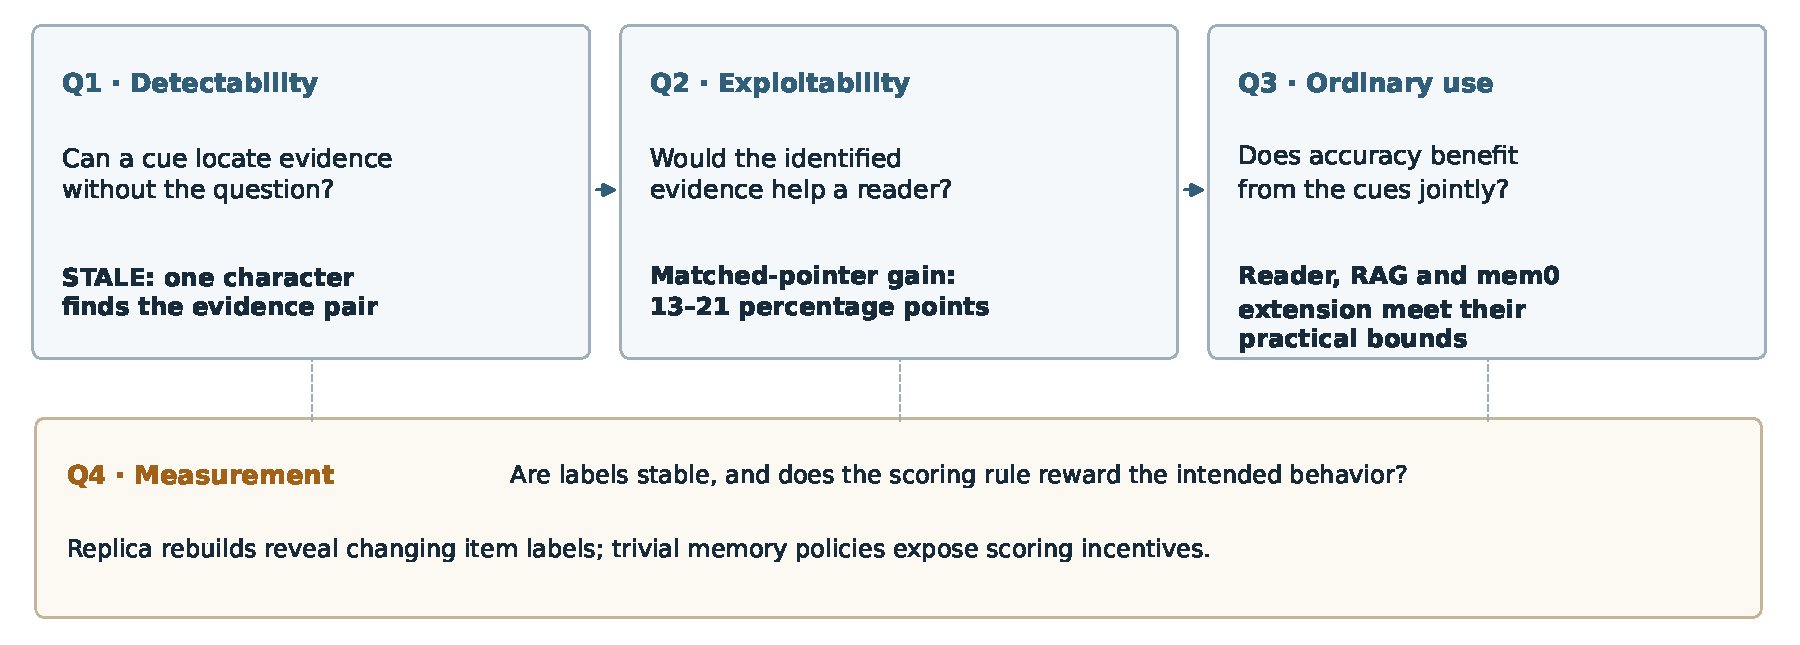
\includegraphics[width=1\linewidth,height=0.72\textheight,keepaspectratio,alt={Overview: four questions about benchmark scores}]{figures/fig0-question-chain.pdf}
\caption*{\textbf{Figure 1. Four questions, with different evidence for each.} A question-blind cue can identify relevant evidence. A pointer experiment asks how much that evidence would help a reader. Removing the cues asks whether tested systems benefit from them in ordinary use. Replica and scoring-rule checks examine how the resulting labels and scores should be interpreted. Each step has its own comparison.}
\end{figure}

\KeepTable{12}{0}

\par\begingroup
\small

\begin{longtable}[]{@{}
  >{\RaggedRight\arraybackslash}p{(\linewidth - 4\tabcolsep) * \real{0.2615}}
  >{\RaggedRight\arraybackslash}p{(\linewidth - 4\tabcolsep) * \real{0.3409}}
  >{\RaggedRight\arraybackslash}p{(\linewidth - 4\tabcolsep) * \real{0.3966}}@{}}
\caption*{\textbf{Four questions at a glance.}}\tabularnewline
\toprule\noalign{}
\begin{minipage}[b]{\linewidth}\RaggedRight
Question
\end{minipage} & \begin{minipage}[b]{\linewidth}\RaggedRight
Short answer
\end{minipage} & \begin{minipage}[b]{\linewidth}\RaggedRight
Key number
\end{minipage} \\
\midrule\noalign{}
\endfirsthead
\toprule\noalign{}
\begin{minipage}[b]{\linewidth}\RaggedRight
Question
\end{minipage} & \begin{minipage}[b]{\linewidth}\RaggedRight
Short answer
\end{minipage} & \begin{minipage}[b]{\linewidth}\RaggedRight
Key number
\end{minipage} \\
\midrule\noalign{}
\endhead
\bottomrule\noalign{}
\endlastfoot
Evidence without the question? & STALE reveals evidence; BEAM matches fair nulls. & STALE: one character \\
Would the cue help? & Yes, versus retrieved-session notes. & +13--21 points; four readers \\
Do systems benefit? & Joint-removal intervals bound net benefits. & Upper bounds: reader ≈3.8, RAG ≈1.6, mem0 extension ≈1.4 points \\
Is measurement stable? & Labels change; forgetting scores can reward wiping. & ≈16\% label disagreement; ≈1-point accuracy standard deviation \\
\end{longtable}

\endgroup

The central finding is a gap between an available shortcut and a demonstrated benefit from ordinary use. STALE's evidence is conspicuously marked, and exact retrieval has value. Joint cue removal nevertheless bounds the net accuracy benefit in the tested systems. Together, these findings connect benchmark construction to measured system behavior.

We make three contributions. First, we combine a question-blind evidence audit with an atlas of retrieval under unrelated questions and fair null baselines. Second, we connect those diagnostics to reader controls, cue-removal experiments, replica checks and scoring-rule tests. Third, we turn the checks into a short benchmark-building checklist and an offline toolkit, memaudit. Appendix I gives the study map and validation summary.

\phantomsection\label{main-2}

\section{2. Related work}\label{related-work}

Question-blind auditing extends established tests of whether a benchmark can be solved from incomplete inputs. Hypothesis-only natural-language inference and question-only reading-comprehension baselines exposed annotation artifacts \citep{Gururangan2018AnnotationArtifacts, Poliak2018HypothesisOnly, KaushikLipton2018ReadingComprehension}. Shortcut-learning studies explain why a successful predictor need not learn the intended task \citep{Geirhos2020ShortcutLearning}, while failed partial-input baselines do not certify artifact-free data \citep{Feng2019Misleading}. Adversarial distractors and contrast sets motivate interventions that change a suspected shortcut \citep{JiangBansal2019Shortcuts, Gardner2020ContrastSets}. Our contribution is to connect evidence detectability, the value of exact retrieval, and accuracy under cue removal without equating them.

Long-history benchmarks include LoCoMo, LongMemEval and STALE \citep{Maharana2024LoCoMo, Wu2025LongMemEval, Chao2026STALE}. They evaluate systems that compress, retrieve or update conversational memory, including Mem0 \citep{Chhikara2025Mem0}. Read\-er behavior also depends on evidence position, distracting context and presentation \citep{Liu2024LostMiddle, Shi2023Distracted, Sclar2024Spurious}. Concurrent work tests memory-size leakage and query-conditioned presentation controls \citep{Mondal2026BeforeAnswering, Jiang2026Presentation, Si2026Render}. We instead begin with question-blind evidence labels and use benchmark-specific nulls before testing downstream behavior. Query-independent document advantages already have a long history in information retrieval \citep{Singhal1996Pivoted, Kraaij2002Priors}.

LLM judges can disagree with humans, prefer particular outputs, and respond to presentation \citep{Zheng2023MTBench, Thakur2024JudgingJudges, Panickssery2024SelfPreference}. Prediction churn and underspecification also show that stable aggregate accuracy can coexist with unstable item predictions \citep{MilaniFard2016Churn, DAmour2022Underspecification}. Our replica study expresses this instability as disagreement and an oracle union over repeated builds; the latter is related to pass-at-k coverage \citep{Chen2021PassAtK}. We use a gain derived from Sharma and Lall's released labels as a reference scale \citep{SharmaLall2026Selection}.

\phantomsection\label{main-3}

\section{3. Setup: each question needs a different comparison}\label{setup-each-question-needs-a-different-comparison}

We measure evidence detectability, retrieval value, ordinary-use accuracy and measurement stability separately. A session is a conversation segment; a turn is one message. The unit being ranked can be a session or a turn, depending on the benchmark. A candidate pool is the set of units available for a particular item. Table 1 summarizes the audited settings.

\begin{table}[tbp]

\caption*{\textbf{Table 1. Benchmark coverage.} This table covers eight benchmarks in all. Seven appear in the evidence audit, which has nine settings because BEAM has three scales. MemOps appears in the atlas only; the atlas replaces Persona\-Mem-v2 with MemOps. These are selected settings with tractable adapters, not a prevalence sample. Construction summaries, populations and adapters are in Appendices A, E and K.}

\small

\begin{tabular}{@{}
  >{\RaggedRight\arraybackslash}p{(\linewidth - 4\tabcolsep) * \real{0.3046}}
  >{\RaggedRight\arraybackslash}p{(\linewidth - 4\tabcolsep) * \real{0.2154}}
  >{\RaggedRight\arraybackslash}p{(\linewidth - 4\tabcolsep) * \real{0.4790}}@{}}
\toprule\noalign{}
\begin{minipage}[b]{\linewidth}\RaggedRight
Benchmark
\end{minipage} & \begin{minipage}[b]{\linewidth}\RaggedRight
Evidence-audit unit
\end{minipage} & \begin{minipage}[b]{\linewidth}\RaggedRight
Construction and coverage
\end{minipage} \\
\midrule\noalign{}
STALE \citep{Chao2026STALE} & Session & Generated, edited evidence mixed with LongMemEval distractors; evidence audit and atlas \\
LoCoMo-Plus \citep{Li2026LoCoMoPlus} & Turn & Generated cue dialogues inserted into LoCoMo hosts; audit and atlas \\
LongMemEval-S \citep{Wu2025LongMemEval} & Session & Simulated evidence with simulated and public-chat filler; audit and atlas \\
BEAM \citep{Tavakoli2025BEAM} & User turn & Generated conversations; contradiction-resolution and knowledge-update labels; audit and atlas \\
HaluMem-Medium \citep{Chen2025HaluMem} & Prefix session & Generated user histories adapted to prefix pools; audit and atlas \\
Persona\-Mem-v2 \citep{Jiang2025PersonaMemV2} & User message & Generated preference conversations; cached subset, audit only \\
LoCoMo \citep{Maharana2024LoCoMo} & Session & Generated, edited conversations; audit and atlas \\
MemOps \citep{Hao2026MemOps} & --- & Evidence conversations mixed with distractors; atlas only \\
\bottomrule\noalign{}
\end{tabular}

\end{table}

\textbf{Question-blind evidence detection.} A detector is question-blind when it never sees the question. Our supervised classifier uses 31 style and role features, excluding question text, evidence identifiers and timestamps. Grouped cross-validation keeps related units together. We report the area under the ROC curve, or AUROC, averaged across candidate pools. A value of .5 is chance discrimination; 1 means perfect separation. This is classification of annotated evidence, not answer correctness. Appendices A and K specify the scored populations, duplicate exclusions and features.

\textbf{Fair nulls for unrelated questions.} A retriever can find an evidence unit even under an unrelated question because that unit is long, has many turns, or occupies a favored position. We therefore compare wrong-question retrieval with uniform chance, chance weighted by nonempty turn count, and matched non-evidence units with similar length, turn count and position. The retriever combines BM25 and dense rankings; a unit's score is its best turn score. The primary outcome is whether any evidence unit appears in the top five. Chance-corrected excess is the average of each item's excess hit rate divided by its remaining room above chance. Matched-placebo comparisons require adequate support: suitable control units must actually exist. Appendix E specifies the nulls and decision rules.

\textbf{The STALE task.} Each of its 400 scenarios contains 50 sessions: an old fact, a later implicit update and 48 distractors. Its three questions test the updated state, resistance to an outdated premise and advice that depends on the update. Reader-pointer experiments use a fixed 100-scenario test split. The reader already sees the full history. A pointer is an added note naming sessions selected by a retriever; the cue pointer instead names the pair found by the character rule. The principal comparison matches the note and the number of named sessions. Cue-removal experiments instead change the input typography and clock times, without adding a pointer.

\textbf{Readers and labels.} The four-vendor comparison uses GLM-5.3-Flash, Gemini 3.8 Flash, GPT-6.1 Sol and Muse Spark 1.3; GPT-6.1 Sol grades correctness for the primary analysis. The pipeline experiments use GLM-5.3-Flash for reading and judging; mem0 also uses it for extraction. Validation compares sampled answers with an additional model's grades, typically Claude Opus 5.5. The replica study rebuilds one bespoke pipeline on LoCoMo and compares the resulting labels. Appendix K summarizes the model and prompt settings.

\textbf{Analysis.} Pre-specified means the design and decision rules were fixed locally before each test run, without a public registration. We assess practical equivalence against a preset tolerance around zero. Bootstrap intervals resample whole scenarios or conversations to preserve dependence among their questions. Holm and Bonferroni adjustments control false positives across families of comparisons. Appendix I gives the study map and validation summary.

\phantomsection\label{main-4}

\section{4. Q1: some benchmarks reveal the evidence without the question}\label{q1-some-benchmarks-reveal-the-evidence-without-the-question}

STALE and LoCoMo-Plus strongly separate evidence from distractors, while BEAM's wrong-question retrieval is equivalent to fair chance. The two findings come from different tests: the first identifies evidence features; the second asks whether unrelated questions retrieve evidence beyond a suitable baseline.

On STALE, the curly-apostrophe rule is exact on the distributed full histories. It selects the evidence pair in all 400 scenarios. This is simpler than training a classifier and shows why evidence construction deserves inspection before a downstream score is interpreted. The classifier also achieves perfect separation on its scored population (Figure 2).

LoCoMo-Plus shows a different stylistic pattern. None of its 758 cue turns contains an exclamation mark, whereas most host turns do. Its multifeature classifier is nearly perfect at distinguishing the two kinds of turn. Recovering every evidence turn for a question is a stricter task than separating the two distributions.

LongMemEval-S is less separable overall. Earlier fits find much stronger separation when evidence is compared with public-chat filler than with simulated filler. This descriptive association is consistent with different construction pipelines leaving different traces. LoCoMo is the weakest setting in the style audit.

\begin{figure}[tbp]
\centering
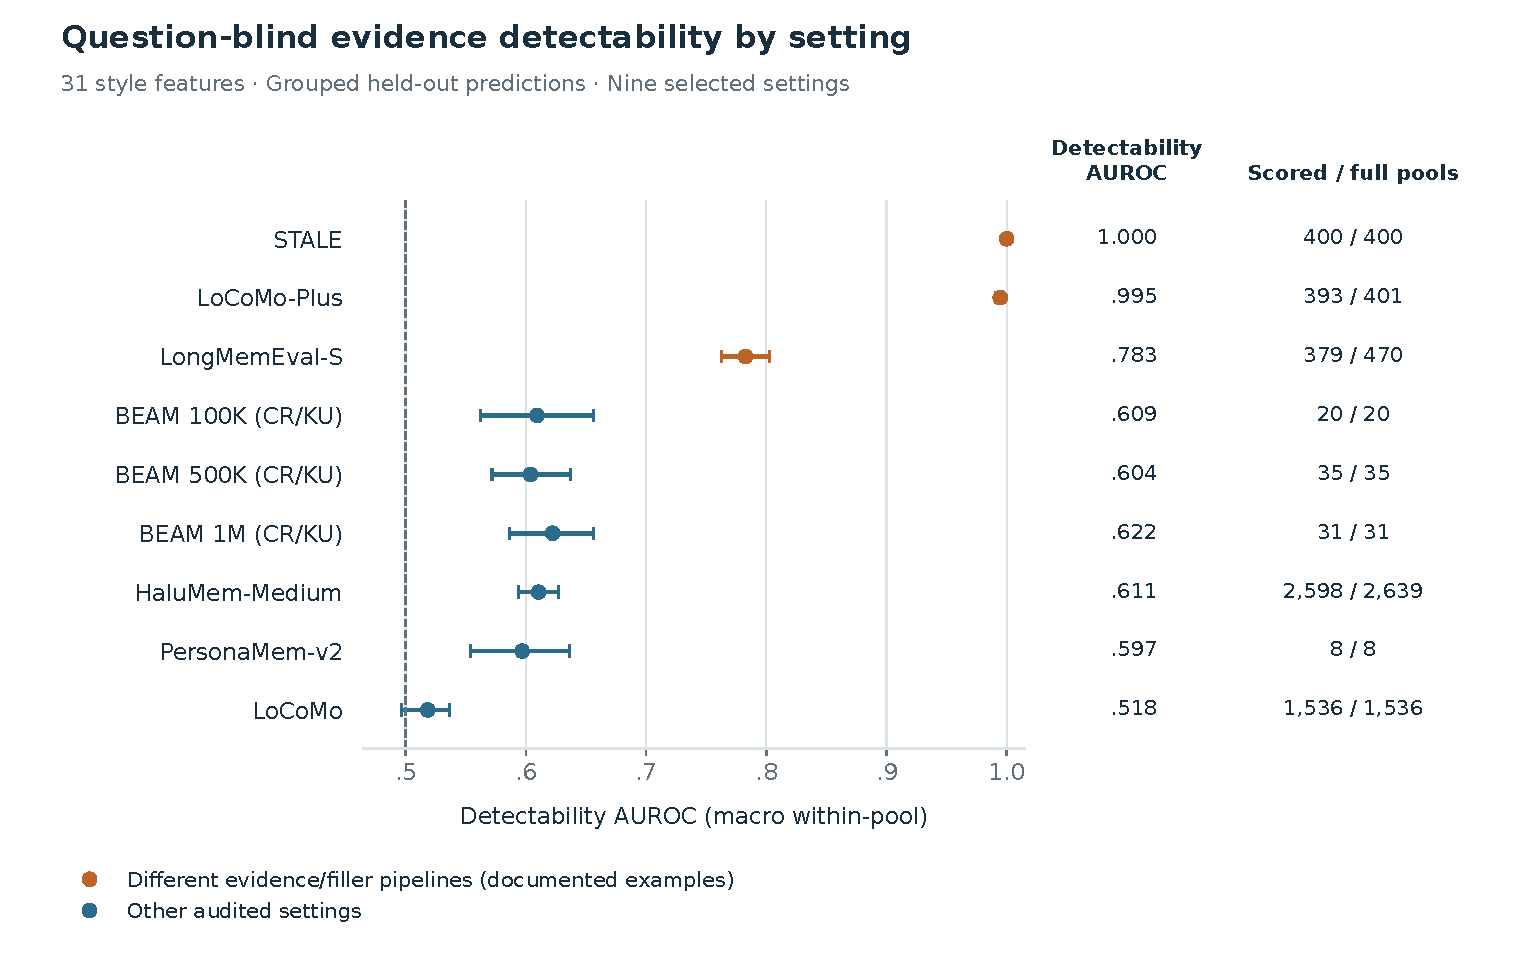
\includegraphics[width=1\linewidth,height=0.72\textheight,keepaspectratio,alt={Figure 2: question-blind evidence detectability}]{figures/fig1-query-blind-auroc.pdf}
\caption*{\textbf{Figure 2. Evidence detectability varies across settings.} Points are macro within-pool AUROCs from 31-feature classifiers on held-out groups after test-duplicate exclusion; bars are saved 95\% group-bootstrap intervals conditional on predictions. The dashed line marks chance. Source-construction colors identify documented differences between evidence and filler pipelines. Appendix A gives the scored populations, including the cached Persona\-Mem-v2 subset and the BEAM population discrepancy.}
\end{figure}

The atlas asks a stricter question about retrieval. In BEAM, unrelated questions retrieve evidence at almost the same rate as turn-weighted chance. Both its primary and matched-placebo comparisons meet the pre-specified equivalence criterion (Table 2; Figure 3). BEAM therefore supplies a negative control for the atlas.

Fair nulls also change LongMemEval-S's interpretation. Its wrong-question hit rate exceeds uniform chance, but weighting units by turn count accounts for much of the excess. A naive uniform baseline would attribute a mechanical opportunity advantage to something more distinctive.

Our HaluMem adaptation illustrates a failure of the audit itself. The pre-specified candidate histories ended at the later of the question's session and the latest evidence session. That rule often put evidence at the end, creating a positional shortcut. The prefix result reflects this adaptation choice. A descriptive check on full histories of the same items removes the cue-dominance flag and places retrieval near its fair null. Appendix E preserves both results.

\begin{table}[tbp]

\caption*{\textbf{Table 2. Selected atlas comparisons.} Rates are percentages for any evidence in the top five. CE is chance-corrected excess over the turn-weighted null. BEAM's rates are item-weighted while its CE weights scales equally; CE is calculated per item, so it cannot in general be reconstructed from the displayed mean rates. The BEAM comparisons meet a ±.03 equivalence bound with Holm adjustment; the remaining rows use descriptive 95\% intervals. Appendix E gives the atlas methods and support checks.}

\small

\begin{tabular}{@{}
  >{\RaggedRight\arraybackslash}p{(\linewidth - 6\tabcolsep) * \real{0.2994}}
  >{\raggedleft\arraybackslash}p{(\linewidth - 6\tabcolsep) * \real{0.2238}}
  >{\raggedleft\arraybackslash}p{(\linewidth - 6\tabcolsep) * \real{0.2296}}
  >{\RaggedRight\arraybackslash}p{(\linewidth - 6\tabcolsep) * \real{0.2462}}@{}}
\toprule\noalign{}
\begin{minipage}[b]{\linewidth}\RaggedRight
Setting /\allowbreak{} comparison
\end{minipage} & \begin{minipage}[b]{\linewidth}\raggedleft
Wrong-question rate
\end{minipage} & \begin{minipage}[b]{\linewidth}\raggedleft
Null or placebo rate
\end{minipage} & \begin{minipage}[b]{\linewidth}\RaggedRight
CE {[}interval{]}
\end{minipage} \\
\midrule\noalign{}
BEAM /\allowbreak{} turn-weighted null & 4.44 & 4.84 & −.004 {[}−.014, .006{]} \\
BEAM /\allowbreak{} matched placebos & --- & --- & −.007 {[}−.020, .006{]} \\
LongMemEval-S /\allowbreak{} turn-weighted null & 22.04 & 21.06 & .011 {[}−.017, .041{]} \\
HaluMem /\allowbreak{} full-history sensitivity & 7.71 & 8.11 & −.005 {[}−.015, .006{]} \\
\bottomrule\noalign{}
\end{tabular}

\end{table}

\begin{figure}[tbp]
\centering
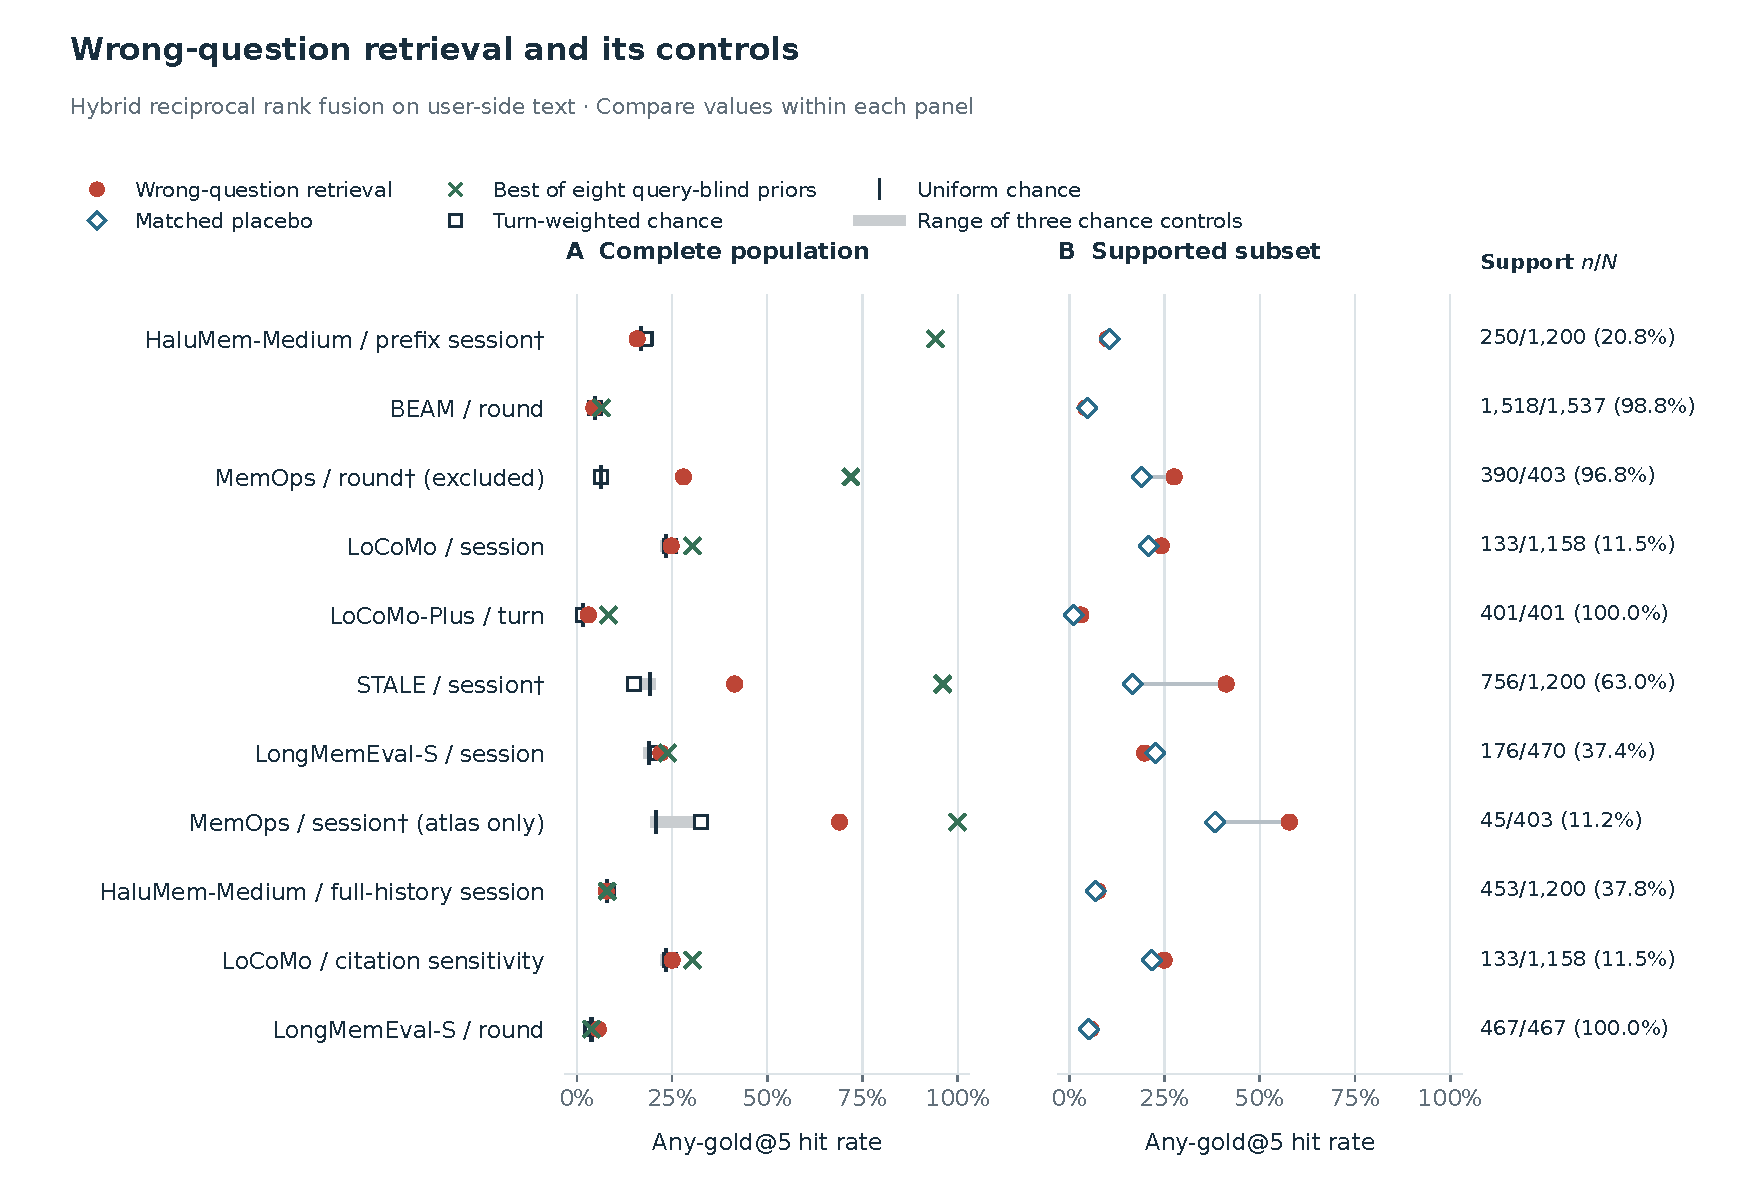
\includegraphics[width=1\linewidth,height=0.72\textheight,keepaspectratio,alt={Figure 3: wrong-question retrieval and its controls}]{figures/fig2-wrong-question-atlas.pdf}
\caption*{\textbf{Figure 3. Wrong-question retrieval needs benchmark-specific controls.} The atlas compares unrelated-question retrieval with query-independent priors and fair nulls. High hit rates can arise from unit structure; the atlas marks cue-dominated rows and insufficient placebo support. Appendices A and E give the populations, estimates and clustering.}
\end{figure}

These results describe evidence detectability and retrieval in the audited settings; they do not estimate effects on answer accuracy.

\phantomsection\label{main-5}

\section{5. Q2: the cue-identified pair is valuable to readers}\label{q2-the-cue-identified-pair-is-valuable-to-readers}

Giving readers STALE's cue-identified evidence improves judged accuracy by 13--21 points over matched two-session retrieval pointers. The reader already receives the full history. What changes is a note telling it which sessions to consult.

The character rule names exactly the old and new evidence sessions. The comparison notes instead name two sessions selected by hybrid or dense retrieval, using the same wording and session count. The character is normalized out of the history shown to the reader. The comparison measures the value of exact retrieval that the cue makes possible.

All four readers show the premium against both matched comparators (Figure 4). The Gemini result comes from a separate successor run. Appendix B gives the paired comparisons.

\begin{figure}[tbp]
\centering
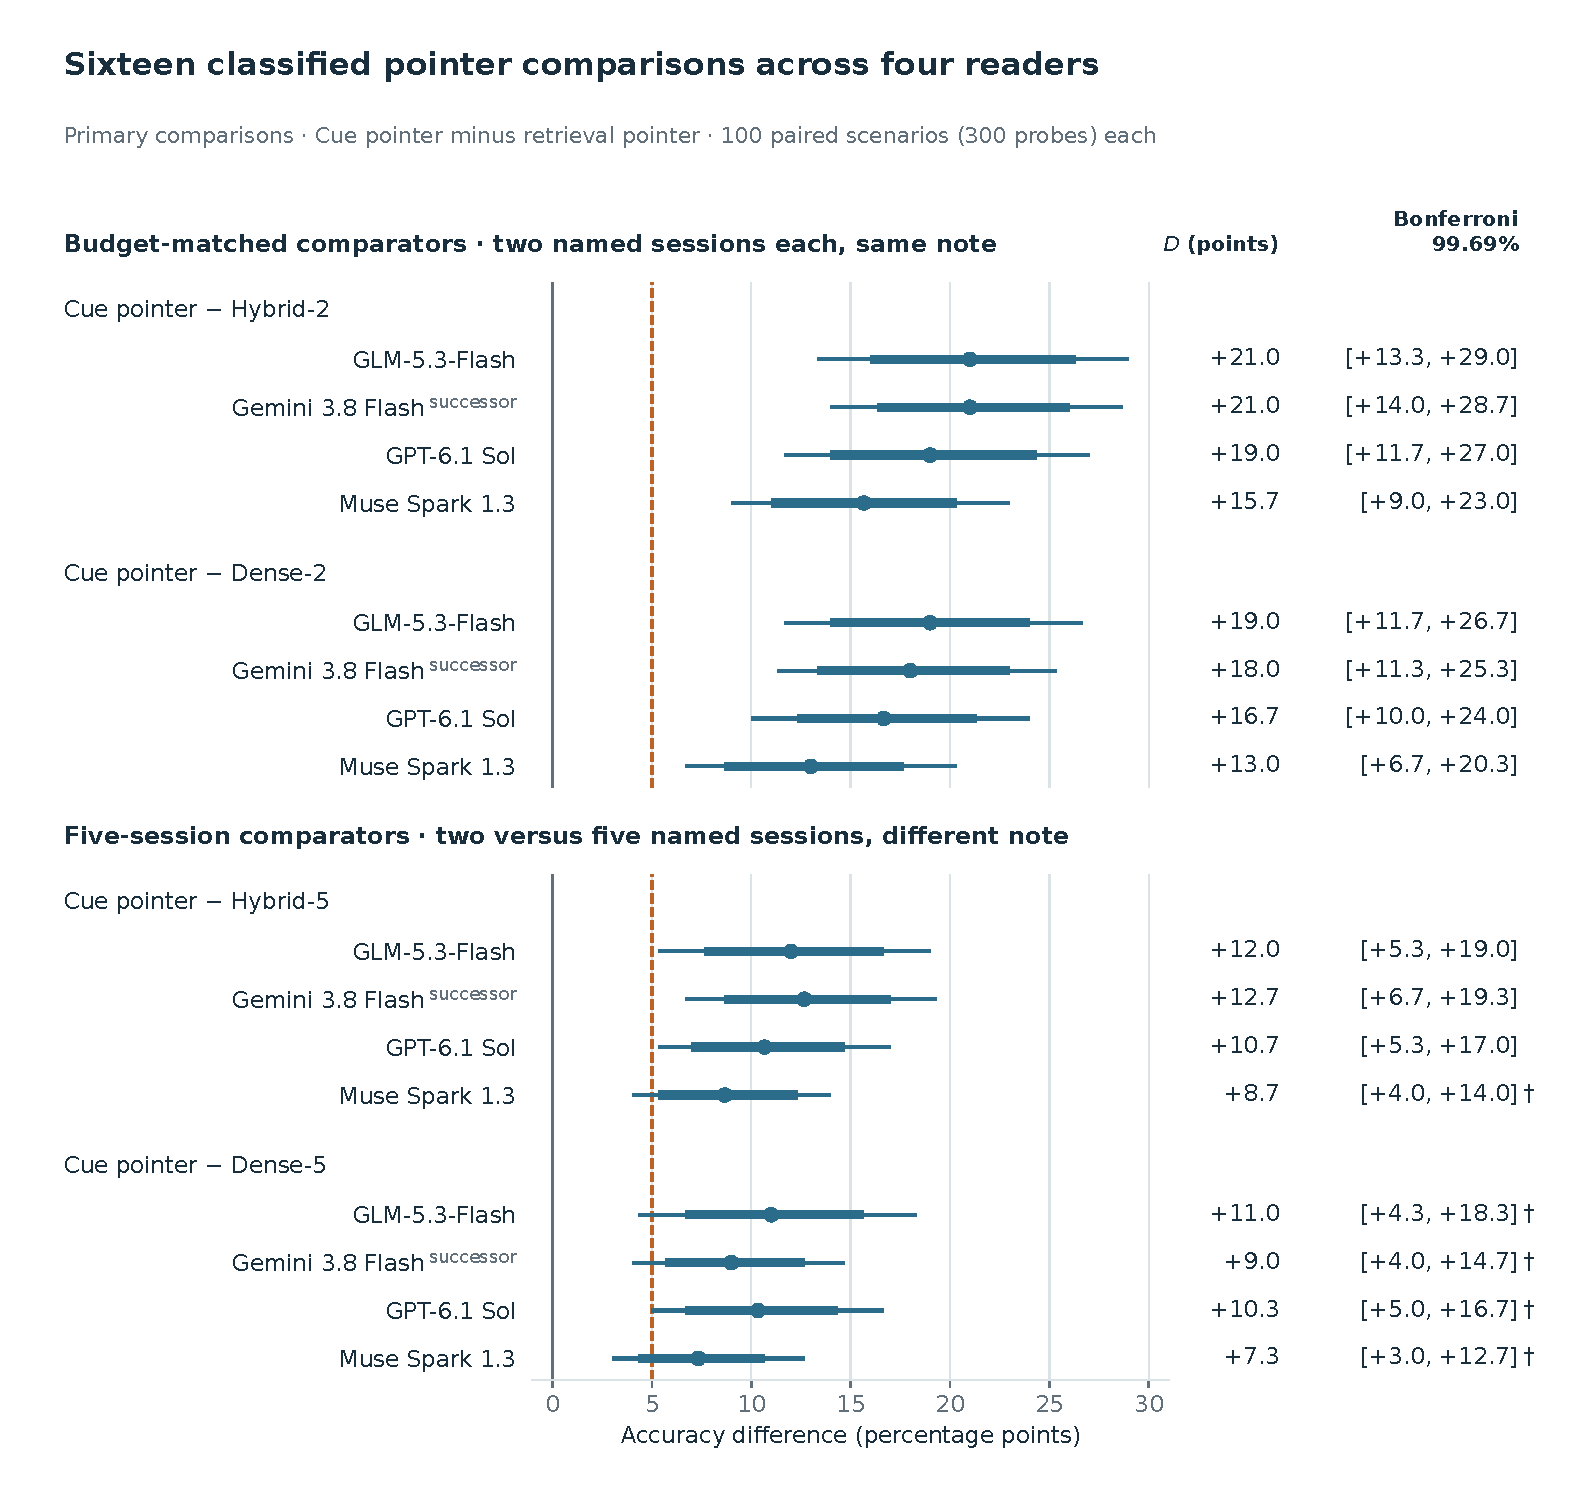
\includegraphics[width=1\linewidth,height=0.72\textheight,keepaspectratio,alt={Figure 4: four-vendor evidence-pointer contrasts}]{figures/fig3-four-vendor-contrasts.pdf}
\caption*{\textbf{Figure 4. Exact evidence beats retrieval pointers across four readers.} Upper panel: cue-pointer minus matched two-session hybrid or dense pointer; lower panel: minus five-session pointers. Each contrast uses 100 paired scenarios and 300 probes. Thick intervals are 95\%; thin intervals are Bonferroni per-contrast 99.69\% intervals for a family of 16 contrasts. All eight two-session comparisons have lower adjusted bounds above five points. Gemini 3.8 Flash results come from the separate successor run. GPT-6.1 Sol supplies the correctness judgments. Detailed model settings, masks and secondary-judge results are in Appendix B.}
\end{figure}

The comparators matter. For every reader, both two-session retrieval pointers score below a generic instruction that names no session. A wrong pointer can misdirect the reader as well as omit relevant evidence. These weak comparators help explain the size of the measured premium.

A cheap instruction control explains much of another large gain. In the original reader experiment, three sentences reminding the reader that facts change, that recent information matters and that a question may contain an outdated premise close about 53\% of the gap between plain reading (no note) and an answer-revealing reference note. That reference note supplies the gold answer and marks the earlier statement as outdated; the cue pointer only names sessions. Most of the extra passes are false-premise rejections, exactly the behavior the scoring rubric rewards. Improving a memory-system score can therefore reflect better task instructions as well as better retrieval or storage.

The evidence-pointer direction survives secondary judging. Regrading the same answers with GLM-5.3-Flash keeps the completed contrasts positive (Appendix B).

A deliberately constructed style ranker also exploits STALE's separability: adding the classifier score to hybrid retrieval raises complete-evidence recall by 34 points. The same construction lowers recall on LongMemEval-S (Appendix D).

The reader premium applies to STALE and the matched retrieval-pointer comparisons, with the character normalized out of the displayed history.

\phantomsection\label{main-6}

\section{6. Q3: joint removal bounds net benefits in three tested settings}\label{q3-joint-removal-bounds-net-benefits-in-three-tested-settings}

For the plain reader, RAG and mem0 extension, the decision intervals exclude a net benefit from the two cues larger than about 3.8, 1.6 and 1.4 percentage points, respectively (Table 3). The cue-removal experiments compare each system on STALE as distributed with the same input after typography is normalized and session clock times are removed while dates remain. These upper bounds and the 13--21-point pointer premium answer different questions: changing the input cues is different from telling the reader where the evidence is.

These studies removed the two cues together; separate removal, as recommended in checklist item 3, remains future work.

Unlike the pointer experiment, these systems receive no hint about where the evidence is. The plain-reader comparison uses a non-official user-only layout, retaining user messages in our session template; official layout means STALE's own session-and-role formatting. The pipeline comparisons use that official layout: a hybrid retrieval-augmented generation pipeline reads retrieved sessions, while the mem0 pipeline reads memories built separately for each condition. Both pipelines use GLM-5.3-Flash. The mem0 system uses version 2.2.1 with user-only ingestion \citep{Mem0Library}. Grading prompts and gold text are identical across pipeline conditions.

\KeepTable{19}{0}

\par\begingroup
\small

\begin{longtable}[]{@{}
  >{\RaggedRight\arraybackslash}p{(\linewidth - 8\tabcolsep) * \real{0.2538}}
  >{\raggedleft\arraybackslash}p{(\linewidth - 8\tabcolsep) * \real{0.1414}}
  >{\RaggedRight\arraybackslash}p{(\linewidth - 8\tabcolsep) * \real{0.2581}}
  >{\RaggedRight\arraybackslash}p{(\linewidth - 8\tabcolsep) * \real{0.1825}}
  >{\RaggedRight\arraybackslash}p{(\linewidth - 8\tabcolsep) * \real{0.1632}}@{}}
\caption*{\textbf{Table 3. Accuracy with the cues minus accuracy after joint removal.} Effects and intervals are percentage points. The reader interval is a 95\% scenario bootstrap; RAG and the first mem0 subset use their Holm-level decision intervals; the mem0 extension uses the wider of its unadjusted 95\% bootstrap and t intervals. The plain reader uses interval inclusion; the pipelines use two one-sided tests (TOST) against the stated bounds. Counts are usable scenarios. The mem0 extension was run on the complementary scenarios after the first subset's inconclusive result. A descriptive pool of 398 scenarios gives +0.71 {[}−1.62, +3.06{]}. Appendices B.3 and L give the analyses.}\tabularnewline
\toprule\noalign{}
\begin{minipage}[b]{\linewidth}\RaggedRight
System
\end{minipage} & \begin{minipage}[b]{\linewidth}\raggedleft
Scenarios
\end{minipage} & \begin{minipage}[b]{\linewidth}\RaggedRight
Difference {[}decision interval{]}
\end{minipage} & \begin{minipage}[b]{\linewidth}\RaggedRight
Practical bound
\end{minipage} & \begin{minipage}[b]{\linewidth}\RaggedRight
Result
\end{minipage} \\
\midrule\noalign{}
\endfirsthead
\toprule\noalign{}
\begin{minipage}[b]{\linewidth}\RaggedRight
System
\end{minipage} & \begin{minipage}[b]{\linewidth}\raggedleft
Scenarios
\end{minipage} & \begin{minipage}[b]{\linewidth}\RaggedRight
Difference {[}decision interval{]}
\end{minipage} & \begin{minipage}[b]{\linewidth}\RaggedRight
Practical bound
\end{minipage} & \begin{minipage}[b]{\linewidth}\RaggedRight
Result
\end{minipage} \\
\midrule\noalign{}
\endhead
\bottomrule\noalign{}
\endlastfoot
Plain Gemini 3.8 Flash reader & 100 & +1.33 {[}−1.17, +3.83{]} & ±5 & Within bound \\
Hybrid RAG, GLM-5.3-Flash & 398 & +0.15 {[}−1.29, +1.60{]} & ±3 & Equivalent \\
mem0 2.2.1, first subset & 150 & +4.30 {[}−0.21, +8.89{]} & ±5 & Inconclusive \\
mem0 2.2.1, extension & 248 & −1.46 {[}−4.33, +1.42{]} & ±5 & Equivalent \\
\end{longtable}

\endgroup

The RAG result meets its pre-specified practical bound. The first mem0 subset remains inconclusive; the extension on complementary scenarios meets ±5 points, with an interval extending beyond ±3 points. Appendix L gives the subset and pooled estimates.

These results bound the net effect of removing typography and clock times together in the tested layouts. Accuracy could remain stable despite cue use, or the effects of the two changes could offset one another. Two end-to-end tests that replaced STALE's distractors were invalid, because judge failures left too many answers ungraded; they give no estimate (Appendix D).

\phantomsection\label{main-7}

\section{7. Q4: stable totals can hide changing labels and flawed incentives}\label{q4-stable-totals-can-hide-changing-labels-and-flawed-incentives}

If labels change between rebuilds of an unchanged system, small cue effects and system comparisons generally become harder to detect from item labels; Q4 asks whether the measurement can support these comparisons. Rebuilding the same memory pipeline changes many item labels while leaving overall accuracy comparatively stable. Separately, a forgetting score can reward deleting useful memory. These are distinct reasons to inspect what a headline score aggregates.

\subsection{Replica labels change more than aggregate accuracy}\label{replica-labels-change-more-than-aggregate-accuracy}

We rebuilt one bespoke GLM-5.3-Flash memory pipeline ten times on four LoCoMo conversations (Figure 5). It uses its own implementation of components modeled on Mem0 \citep{Chhikara2025Mem0}. Pairs of builds disagree on about 16\% of LLM-judged labels on average, while run-level accuracy has a standard deviation of about one point. Aggregation across many questions allows those two facts to coexist.

A per-question oracle union illustrates the potential effect of selecting successful runs after the fact. It chooses a correct label if either replica has one. Its gain over the pair mean is exactly half the pair's disagreement. This diagnostic selector uses the correctness labels to choose between replicas.

\begin{figure}[tbp]
\centering
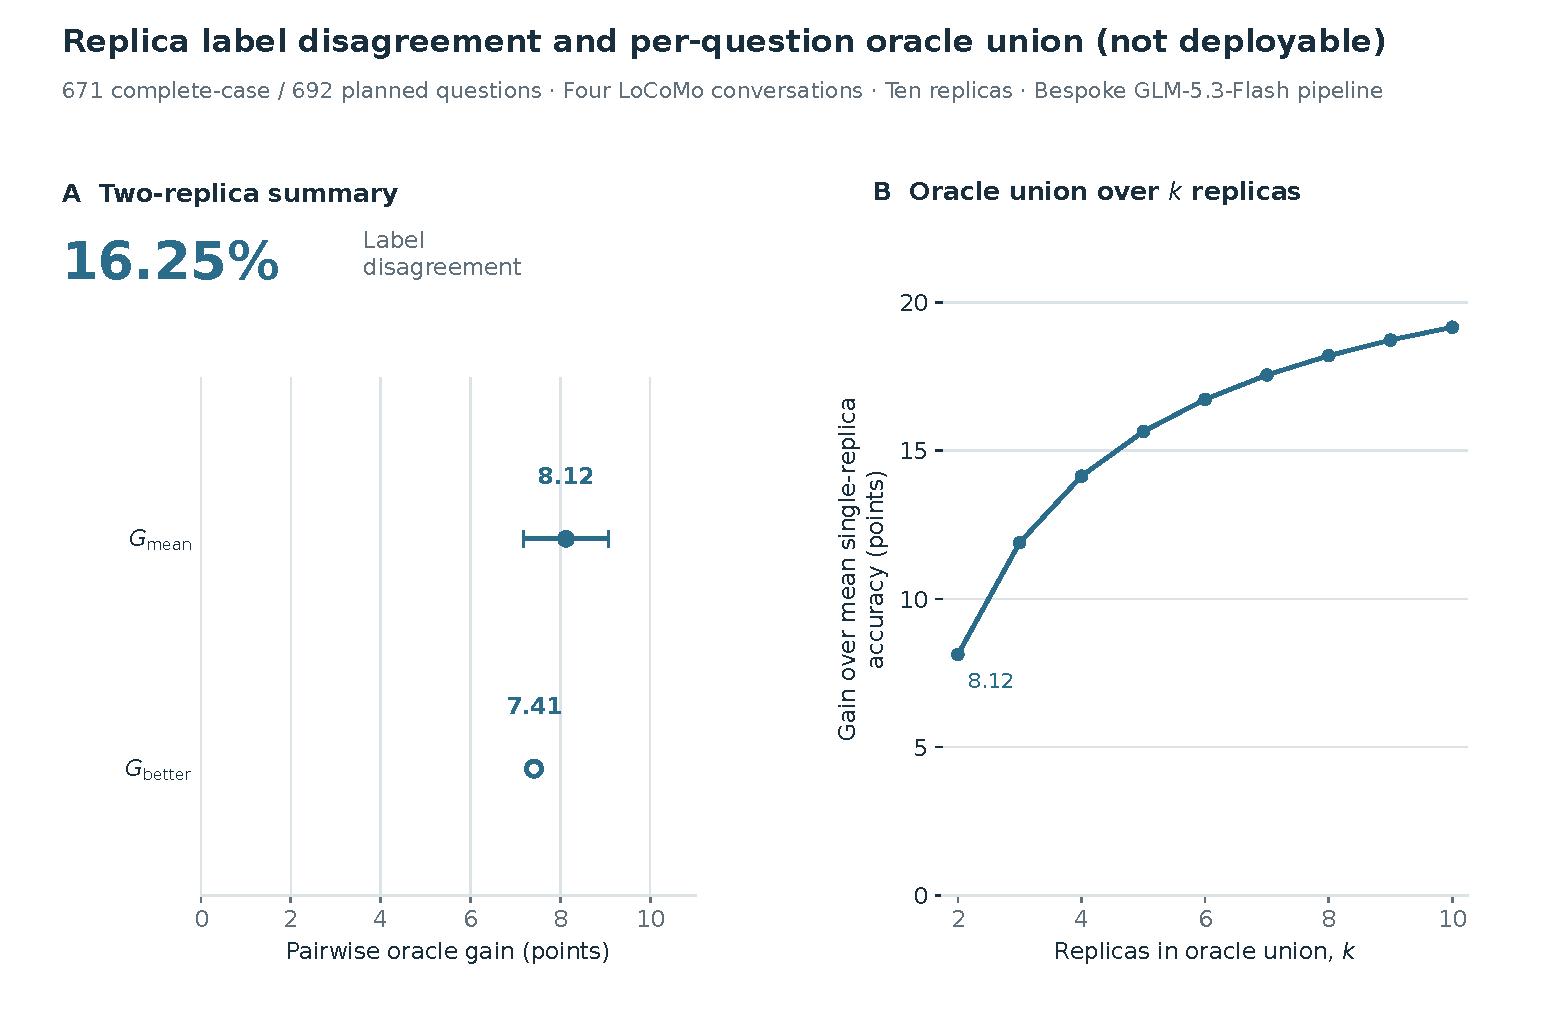
\includegraphics[width=1\linewidth,height=0.72\textheight,keepaspectratio,alt={Figure 5: replica disagreement and oracle union}]{figures/fig6-replica-oracle.pdf}
\caption*{\textbf{Figure 5. Item-level disagreement and an unattainable selection advantage.} The primary replica analysis has 671 complete-case questions from four conversations and ten builds. Mean pairwise disagreement is 16.25\%, giving an oracle gain over the pair mean of 8.12 points {[}7.18, 9.07{]}; the interval is conditional on these conversations. The gain over the better member is 7.41 points without an interval. The exploratory curve averages oracle unions over replica subsets of sizes two through ten. Replica pairs share members. Accuracy's SD is 1.04 points. Appendix C gives the different complete-case masks.}
\end{figure}

The practical implication is to compare a proposed system change with the variation produced by rebuilding an unchanged system, reporting both item-level disagreement and aggregate accuracy.

\subsection{Judge validation and an author sanity check}\label{judge-validation-and-an-author-sanity-check}

Regrading sampled answers with additional models shows substantial agreement with the original labels. Appendices C and F summarize the checks.

As a sanity check, the author (aware of the design, with condition labels hidden) graded a sample. The judge agreed with the author on 45 of 50 replica answers, and 10 of 15 sampled disagreements were real correctness differences (Appendix J).

\subsection{ForgetEval's score can reward wiping memory}\label{forgetevals-score-can-reward-wiping-memory}

ForgetEval scores whether targeted information has been removed from memory \citep{Yang2026ForgetEval}. A template case is a test item generated from a preset forgetting pattern; storing nothing is the trivial policy that leaves the memory empty. On ForgetEval, a policy that wipes memory and inserts a replacement passes 750 of 1,000 template cases, compared with 350 for storing nothing. This happens because the public rule can reward removing targeted content without adequately penalizing lost retained content. A successful deletion score is therefore not enough: forgetting should be measured alongside preservation of information that is meant to remain.

Appendix G gives the policy definitions and score comparisons.

The replica estimates are conditional on four conversations and the tested pipeline, while the ForgetEval result applies to its public scoring rule.

\phantomsection\label{main-8}

\section{8. Checklist for benchmark builders}\label{checklist-for-benchmark-builders}

The checks below separate available shortcuts, actual score effects and measurement failures.

\begin{enumerate}
\def\labelenumi{\arabic{enumi}.}
\tightlist
\item
  \textbf{Inspect evidence before testing systems.} Scan single characters, length, turn count and position. Record how evidence and filler were produced, and check whether data adaptation itself creates a shortcut. Evaluate detectors on grouped held-out data and disclose duplicate exclusions.
\item
  \textbf{Use baselines that match the opportunity to succeed.} Compare wrong-question retrieval with turn-weighted chance and matched placebos. Match pointer notes and session counts. Include a simple task-instruction control before attributing a reader gain to memory.
\item
  \textbf{Test score dependence with a targeted intervention.} Preserve intended task difficulty where possible. Remove suspect cues separately as well as jointly, keep rendering controlled, and report retrieval support separately from answer accuracy. A valuable shortcut need not be used by the system being tested.
\item
  \textbf{Measure variation and validate labels.} Rebuild unchanged pipelines, report item disagreement as well as aggregate spread, and validate judges on the answers being compared. Report validation quality alongside the comparisons.
\item
  \textbf{Test the scoring rule with trivial policies.} Try storing nothing and wiping memory. Report forgotten-set closure and collateral loss separately. Tie each conclusion to a comparison that could falsify it, and state the population and analysis choices clearly.
\end{enumerate}

\phantomsection\label{main-9}

\section{9. Limitations}\label{limitations}

The audit covers selected benchmark settings and implementations. Weak style discrimination leaves room for other detectors, and associations between construction pipelines and style are descriptive. Cue-removal results apply to STALE, the tested layouts and the two cues changed together. Clock times can also carry legitimate temporal information.

The correctness labels depend on model judgments, and some experiments use the same model family for reading and grading. The author sanity check uses one grader, not a panel. The replica estimates are conditional on four conversations; shared scenarios, questions and replicas limit extrapolation to other populations.

Several experiments reuse populations. The practical margins define the tolerance used in these comparisons. Fresh populations, separate cue interventions and independent human grading would strengthen the evidence.

\phantomsection\label{main-10}

\section{10. Conclusion}\label{conclusion}

STALE contains an exact question-blind evidence cue, and supplying the identified evidence helps readers. Joint removal bounds net accuracy benefits for the plain reader, RAG and mem0 extension within their pre-specified practical margins. Replica checks and null memory policies expose further ways a headline score can hide item instability or reward unintended behavior. Benchmark builders should test each of these links. The checklist and memaudit make several of the checks inexpensive to run.

\phantomsection\label{main-release}

\section*{Release, licenses and toolkit}\label{release-licenses-and-toolkit}
\addcontentsline{toc}{section}{Release, licenses and toolkit}

The existing \href{https://github.com/ozgurugurlu/memaudit}{memaudit 0.1.0 release} is an Apache-2.0 offline CPU toolkit for question-blind unit audits, wrong-question retrieval with fair nulls, ForgetEval null policies and numeric replica replay. It runs no language model. Its default retriever is BM25; a hybrid option needs a local dense encoder. Documented checks reproduce selected STALE and LoCoMo-Plus measurements, but the package is not a full reproduction of this paper's model experiments or confirmatory atlas rows.

The distribution contains code, documentation, invented examples and aggregate statistics; benchmark text, raw model outputs and per-item outcomes are excluded. Appendix H summarizes source licenses and release boundaries.

\clearpage
\bibliographystyle{plainnat}
\bibliography{references}

\clearpage
\phantomsection
\pdfbookmark[0]{Supplementary appendix}{public-appendix}
\begin{center}
{\LARGE\bfseries Supplementary appendix}\par\vspace{0.6em}
{\large Finding the Evidence Without the Question}\par
\vspace{0.4em}{\normalsize Özgür Uğurlu}\par
\end{center}
\vspace{0.5em}
This appendix gives the methods and aggregate results behind the four research questions. Table I1 maps descriptive study names to study codes. GLM abbreviates GLM-5.3-Flash.

\phantomsection\label{appendix-a}

\section{A. Evidence detectability and audit scope}\label{a.-evidence-detectability-and-audit-scope}

The question-blind audit fits a histogram gradient-boosting classifier to 31 typography, format, length and lexical features (K.2), without questions, evidence identifiers or timestamps. Five-fold cross-validation keeps conversations, users or hosts together. Test rows whose unit text occurs in training are excluded; pools need both classes after exclusion. Detectability AUROC is the unweighted mean of within-pool AUROCs. The 95\% intervals use 2,000 group-bootstrap resamples of saved predictions, conditional on the fitted models. BEAM uses contradiction-resolution and knowledge-update labels only.

\KeepTable{16}{0}

\par\begingroup
\small

\begin{longtable}[]{@{}
  >{\RaggedRight\arraybackslash}p{(\linewidth - 6\tabcolsep) * \real{0.1809}}
  >{\RaggedRight\arraybackslash}p{(\linewidth - 6\tabcolsep) * \real{0.1809}}
  >{\raggedleft\arraybackslash}p{(\linewidth - 6\tabcolsep) * \real{0.2819}}
  >{\RaggedRight\arraybackslash}p{(\linewidth - 6\tabcolsep) * \real{0.3553}}@{}}
\caption*{\textbf{Table A1. Question-blind detectability in the audited populations.} Counts give pools before exclusion and those retaining both classes. Intervals are conditional 95\% group-bootstrap intervals. BEAM 1M has 35 source conversations and 31 eligible ones.}\tabularnewline
\toprule\noalign{}
\begin{minipage}[b]{\linewidth}\RaggedRight
Setting
\end{minipage} & \begin{minipage}[b]{\linewidth}\RaggedRight
Evidence unit
\end{minipage} & \begin{minipage}[b]{\linewidth}\raggedleft
Pools before exclusions → scored
\end{minipage} & \begin{minipage}[b]{\linewidth}\RaggedRight
Detectability AUROC (macro within-pool) {[}95\% interval{]}
\end{minipage} \\
\midrule\noalign{}
\endfirsthead
\toprule\noalign{}
\begin{minipage}[b]{\linewidth}\RaggedRight
Setting
\end{minipage} & \begin{minipage}[b]{\linewidth}\RaggedRight
Evidence unit
\end{minipage} & \begin{minipage}[b]{\linewidth}\raggedleft
Pools before exclusions → scored
\end{minipage} & \begin{minipage}[b]{\linewidth}\RaggedRight
Detectability AUROC (macro within-pool) {[}95\% interval{]}
\end{minipage} \\
\midrule\noalign{}
\endhead
\bottomrule\noalign{}
\endlastfoot
STALE & Session & 400 → 400 & 1.000 {[}1.000, 1.000{]} \\
LoCoMo-Plus & Turn & 401 → 393 & .995 {[}.991, .997{]} \\
LongMemEval-S & Session & 470 → 379 & .783 {[}.763, .803{]} \\
BEAM 100K & User turn & 20 → 20 & .609 {[}.562, .656{]} \\
BEAM 500K & User turn & 35 → 35 & .604 {[}.572, .637{]} \\
BEAM 1M & User turn & 35 (31 eligible) → 31 & .622 {[}.586, .656{]} \\
HaluMem-Medium & Prefix session & 2,639 → 2,598 & .611 {[}.594, .627{]} \\
Persona\-Mem-v2 & User message & 8 → 8 & .597 {[}.554, .636{]} \\
LoCoMo & Session & 1,536 → 1,536 & .518 {[}.496, .537{]} \\
\end{longtable}

\endgroup

For STALE, the character U+2019 identifies all 800 evidence sessions and none of the 19,200 distractor sessions. Duplicate exclusion removes 10,540 distractor rows; Table A1's AUROC describes the retained rows. LongMemEval-S scores .752 {[}.732, .769{]} on all 470 pools when duplicates are instead purged from training. BEAM 1M excludes four conversations with nonmonotonic or duplicated message identifiers. Persona\-Mem-v2 uses eight cached histories whose selection from 200 personas was not recorded.

\phantomsection\label{appendix-b}

\section{B. Reader interventions}\label{b.-reader-interventions}

Each ladder arm supplies the full history and question. Pointer notes name sessions and instruct the reader to prefer newer information when statements conflict. The artifact pointer identifies the evidence pair using U+2019 before typography is normalized out of the reader's history; retrieval pointers use the question. Thus the intervention supplies the cue's retrieval result, not the visible character itself.

\subsection{B.1. Original ladder (S10b)}\label{b.1.-original-ladder-s10b}

The original test uses 100 STALE scenarios and 300 probes with GLM-5.3-Flash as reader and judge. Accuracy is 63.7\% for plain reading, 83.0\% with the generic instruction, 86.0\% with hybrid-5, 98.0\% with the artifact pointer and 100.0\% with the answer-revealing oracle note. The artifact-minus-hybrid difference is +12.0 points {[}95\% interval +8.0, +16.0{]}, Holm p = \(5.7 \times 10^{-10}\). The rule requires an estimate ≥5, lower bound \textgreater0 and adjusted McNemar p \textless{} .05. Generic instructions raise false-premise accuracy from 28.0\% to 79.0\%. The two pointers differ in session count as well as identity.

\phantomsection\label{appendix-b2}

\subsection{B.2. Three-reader ladder (S10c)}\label{b.2.-three-reader-ladder-s10c}

The same 100 scenarios were reused for Gemini 3.8 Flash, Gemini 3.5 Flash-Lite and a fresh GLM anchor. Nine arms include one-, two- and five-session notes, with 35, 46 and 79 tokens. The four primary artifact-minus-five-session contrasts are +14.0 and +7.0 points for Gemini 3.8 Flash, and +19.0 and +17.3 for Flash-Lite (hybrid, then dense). All are supported under Holm adjustment; all but Gemini 3.8 Flash versus dense-5 have adjusted lower bounds above +5. The estimator averages paired probe differences within scenarios, then scenarios equally. It uses 10,000 bootstrap resamples, 10,000 sign flips and 98.75\% Bonferroni per-contrast intervals.

\subsection{B.3. Joint cue removal for a plain reader (S18)}\label{b.3.-joint-cue-removal-for-a-plain-reader-s18}

S18 tests a plain Gemini 3.8 Flash reader at temperature 1.0 and default thinking on the same 100 scenarios. RAW retains original typography and full timestamps; DECUE normalizes typography and removes clock time while retaining dates. Both use user-only histories and identical normalized probes. DECUE equals the earlier plain prompt. Each probe has two draws per arm, scheduled ABBA with balanced starting arm. GPT-6.1 Sol at medium reasoning judges all 1,200 reads in 400 calls.

RAW minus DECUE is +1.33 points {[}−1.17, +3.83{]}, sign-flip p = .362. A scenario bootstrap with 10,000 resamples supplies the 95\% interval. Practical equality requires this interval inside {[}−5, +5{]}; the result meets that rule. This is interval inclusion, not TOST. All 300 probes are complete. Validation is inherited from S17 Part B. The two cues were removed together, in the non-official user-only layout.

\subsection{B.4. Four-vendor matched-pointer ladder (S19)}\label{b.4.-four-vendor-matched-pointer-ladder-s19}

S19 adds two-session hybrid and dense pointers with the artifact pointer's same 46-token note, while retaining five-session comparators. The nine arms also include plain, generic, oracle and gold-pair-plus-three. GLM-5.3-Flash, Gemini 3.8 Flash, GPT-6.1 Sol and Muse Spark 1.3 (standard tier) run at temperature 1.0 and vendor-specific ``high'' reasoning. GPT-6.1 Sol at medium reasoning judges all readers, including its own family.

Byte-identical requests share one read: 2,375 distinct reads per reader for 2,700 nominal outcomes. Scenario blocks follow an 18-row Williams design. A reader needs ≥98\% valid outcomes among the 2,400 non-gold-pair-plus-three units, with terminal reads scored incorrect. The primary family has 16 scenario-mean contrasts, 100,000 bootstrap resamples and 10,000 sign flips. Holm-adjusted p \textless{} .05, estimate ≥5 and lower bound \textgreater0 define support; the stronger result requires a lower bound \textgreater5. Intervals are 99.69\% Bonferroni per-contrast intervals, targeting nominal 95\% family coverage.

\subsection{B.5. Gemini successor and completed contrasts (S19b)}\label{b.5.-gemini-successor-and-completed-contrasts-s19b}

Three S19 readers completed; Gemini's stopped run was replaced only in the family display by its separately specified S19b run. That run uses fresh reads and its own passing validation, with the same split and arms. Table B1 joins its four decisions with the twelve unchanged S19 decisions. All completed contrasts have permutation p = 1/\allowbreak{}10,001 and Holm p = .0016. All eight matched two-session contrasts have adjusted lower bounds above +5. Both two-session retrieval-pointer arms score below the generic instruction for every completed reader.

\par\begingroup
\small

\begin{longtable}[]{@{}
  >{\RaggedRight\arraybackslash}p{(\linewidth - 6\tabcolsep) * \real{0.3143}}
  >{\RaggedRight\arraybackslash}p{(\linewidth - 6\tabcolsep) * \real{0.2072}}
  >{\raggedleft\arraybackslash}p{(\linewidth - 6\tabcolsep) * \real{0.2072}}
  >{\RaggedRight\arraybackslash}p{(\linewidth - 6\tabcolsep) * \real{0.2702}}@{}}
\caption*{\textbf{Table B1. Completed primary contrasts.} Artifact pointer minus comparator, percentage points, 100 scenarios and 300 probes each. Intervals are 99.69\% Bonferroni per-contrast intervals. All contrasts meet the support rule in B.4; the eight two-session comparisons have adjusted lower bounds above +5.}\tabularnewline
\toprule\noalign{}
\begin{minipage}[b]{\linewidth}\RaggedRight
Read\-er
\end{minipage} & \begin{minipage}[b]{\linewidth}\RaggedRight
Comparator
\end{minipage} & \begin{minipage}[b]{\linewidth}\raggedleft
Difference
\end{minipage} & \begin{minipage}[b]{\linewidth}\RaggedRight
Adjusted interval
\end{minipage} \\
\midrule\noalign{}
\endfirsthead
\toprule\noalign{}
\begin{minipage}[b]{\linewidth}\RaggedRight
Read\-er
\end{minipage} & \begin{minipage}[b]{\linewidth}\RaggedRight
Comparator
\end{minipage} & \begin{minipage}[b]{\linewidth}\raggedleft
Difference
\end{minipage} & \begin{minipage}[b]{\linewidth}\RaggedRight
Adjusted interval
\end{minipage} \\
\midrule\noalign{}
\endhead
\bottomrule\noalign{}
\endlastfoot
GLM-5.3-Flash & Hy\-brid-\allowbreak{}2 & +21.0 & {[}+13.3, +29.0{]} \\
GLM-5.3-Flash & Dense-2 & +19.0 & {[}+11.7, +26.7{]} \\
GLM-5.3-Flash & Hy\-brid-\allowbreak{}5 & +12.0 & {[}+5.3, +19.0{]} \\
GLM-5.3-Flash & Dense-5 & +11.0 & {[}+4.3, +18.3{]} \\
Gemini 3.8 Flash (S19b) & Hy\-brid-\allowbreak{}2 & +21.0 & {[}+14.0, +28.7{]} \\
Gemini 3.8 Flash (S19b) & Dense-2 & +18.0 & {[}+11.3, +25.3{]} \\
Gemini 3.8 Flash (S19b) & Hy\-brid-\allowbreak{}5 & +12.7 & {[}+6.7, +19.3{]} \\
Gemini 3.8 Flash (S19b) & Dense-5 & +9.0 & {[}+4.0, +14.7{]} \\
GPT-6.1 Sol & Hy\-brid-\allowbreak{}2 & +19.0 & {[}+11.7, +27.0{]} \\
GPT-6.1 Sol & Dense-2 & +16.7 & {[}+10.0, +24.0{]} \\
GPT-6.1 Sol & Hy\-brid-\allowbreak{}5 & +10.7 & {[}+5.3, +17.0{]} \\
GPT-6.1 Sol & Dense-5 & +10.3 & {[}+5.0, +16.7{]} \\
Muse Spark 1.3 & Hy\-brid-\allowbreak{}2 & +15.7 & {[}+9.0, +23.0{]} \\
Muse Spark 1.3 & Dense-2 & +13.0 & {[}+6.7, +20.3{]} \\
Muse Spark 1.3 & Hy\-brid-\allowbreak{}5 & +8.7 & {[}+4.0, +14.0{]} \\
Muse Spark 1.3 & Dense-5 & +7.3 & {[}+3.0, +12.7{]} \\
\end{longtable}

\endgroup

GLM-5.3-Flash rejudging retains positive artifact-pointer contrasts against every comparator for the completed readers. Gemini's secondary estimates are +20.33, +15.33, +12.67 and +8.33 points against hybrid-2, dense-2, hybrid-5 and dense-5. These are descriptive and do not replace the binding decisions.

\phantomsection\label{appendix-c}

\section{C. Replicas and judge sensitivity}\label{c.-replicas-and-judge-sensitivity}

\phantomsection\label{appendix-c1}

\subsection{C.1. Replica study (S11)}\label{c.1.-replica-study-s11}

S11 rebuilds a bespoke GLM-5.3-Flash fact store ten times from each conversation (K.7). Extraction temperature is .7; reading and judging use temperature 0. The test has four LoCoMo conversations and 692 questions, with 6,901 valid judged answers out of 6,920 planned. There are 680 questions with all ten replica labels. Oracle gain uses 671 questions complete for the extra-reader and raw-turn controls; the variance model uses 675, and the zero-temperature control 677.

For binary labels, oracle union gain over the pair mean is exactly half pairwise disagreement: \(G_{\mathrm{mean}}=d/2\) in points when d is percent. Intervals resample questions and replicas conditional on the four conversations. The oracle selects on correctness labels and measures coverage across builds.

\KeepTable{12}{0}

\par\begingroup
\small

\begin{longtable}[]{@{}
  >{\RaggedRight\arraybackslash}p{(\linewidth - 2\tabcolsep) * \real{0.5949}}
  >{\RaggedRight\arraybackslash}p{(\linewidth - 2\tabcolsep) * \real{0.4041}}@{}}
\caption*{\textbf{Table C1. Replica results.} The variance model uses extra reader/\allowbreak{}judge passes on one designated store; the zero-temperature control has three stores.}\tabularnewline
\toprule\noalign{}
\begin{minipage}[b]{\linewidth}\RaggedRight
Quantity
\end{minipage} & \begin{minipage}[b]{\linewidth}\RaggedRight
Result
\end{minipage} \\
\midrule\noalign{}
\endfirsthead
\toprule\noalign{}
\begin{minipage}[b]{\linewidth}\RaggedRight
Quantity
\end{minipage} & \begin{minipage}[b]{\linewidth}\RaggedRight
Result
\end{minipage} \\
\midrule\noalign{}
\endhead
\bottomrule\noalign{}
\endlastfoot
Pairwise label disagreement & 16.25\% \\
Oracle gain over pair mean & 8.12 points {[}7.18, 9.07{]} \\
Oracle gain over better member & 7.41 points \\
Write-run accuracy SD, net of reader/\allowbreak{}judge noise & 1.04 points {[}0.65, 1.39{]} \\
Median fact-set Jaccard & .701 \\
Oracle gain at requested zero extraction temperature & 8.27 points \\
Judge-free containment gain & 4.54 points \\
\end{longtable}

\endgroup

\phantomsection\label{appendix-c2}

\phantomsection\label{appendix-c4}

\subsection{C.2. Second judge on pointer answers (S17 Parts B and B2)}\label{c.2.-second-judge-on-pointer-answers-s17-parts-b-and-b2}

GPT-6.1 Sol passes validation on S10c's 87-item packet and rejudges 2,700 pointer outcomes. The four primary contrasts remain supported: +12.67 and +7.67 points for Gemini 3.8 Flash, +17.33 and +16.33 for Flash-Lite, against hybrid-5 and dense-5 respectively. It uses S10c's estimator and 98.75\% intervals. Model family and temperature change together; this is a sensitivity analysis on the same answers.

\phantomsection\label{appendix-d}

\section{D. Counterfactual retrieval}\label{d.-counterfactual-retrieval}

S15a replaces distractors while fixing questions, evidence, session counts, positions and dates. ORIG-N is the normalized original history; CF-SOURCE uses evidence sessions from other scenarios on STALE and simulated sessions from other questions on LongMemEval-S. CF-STYLE rewrites distractors and falls back to original text for failed rewrites. The primary outcome is hybrid all-gold@5. A three-test Holm family uses the wider of a 10,000-draw cluster-bootstrap and cluster-mean t interval. Positive effects require adjusted lower bound \textgreater0 and estimate ≥5; the equivalence margin is ±3. Partial manipulations keep p = 1 slots and exploratory contrasts.

\KeepTable{10}{0}

\par\begingroup
\small

\begin{longtable}[]{@{}
  >{\RaggedRight\arraybackslash}p{(\linewidth - 4\tabcolsep) * \real{0.3890}}
  >{\raggedleft\arraybackslash}p{(\linewidth - 4\tabcolsep) * \real{0.2565}}
  >{\RaggedRight\arraybackslash}p{(\linewidth - 4\tabcolsep) * \real{0.3535}}@{}}
\caption*{\textbf{Table D1. Retrieval replacement contrasts.} ORIG-N minus replacement, points. STALE uses 400 scenarios and 1,200 probes; LongMemEval-S uses 470 questions. The STALE source-swap contrast is positive; the style-rewrite and LongMemEval-S contrasts remain exploratory because their manipulation checks are partial.}\tabularnewline
\toprule\noalign{}
\begin{minipage}[b]{\linewidth}\RaggedRight
Replacement
\end{minipage} & \begin{minipage}[b]{\linewidth}\raggedleft
Difference
\end{minipage} & \begin{minipage}[b]{\linewidth}\RaggedRight
Holm-level interval
\end{minipage} \\
\midrule\noalign{}
\endfirsthead
\toprule\noalign{}
\begin{minipage}[b]{\linewidth}\RaggedRight
Replacement
\end{minipage} & \begin{minipage}[b]{\linewidth}\raggedleft
Difference
\end{minipage} & \begin{minipage}[b]{\linewidth}\RaggedRight
Holm-level interval
\end{minipage} \\
\midrule\noalign{}
\endhead
\bottomrule\noalign{}
\endlastfoot
STALE CF-SOURCE & +12.58 & {[}+9.64, +15.53{]} \\
STALE CF-STYLE & −0.25 & {[}−1.67, +1.17{]} \\
LongMemEval-S CF-SOURCE & +1.06 & {[}−0.37, +2.55{]} \\
\end{longtable}

\endgroup

The manipulation check requires question-blind AUROC ≤ .60 and upper 95\% bound ≤ .65. STALE CF-SOURCE passes at .513 {[}.492, .536{]}; CF-STYLE and LongMemEval-S CF-SOURCE fail at 1.000 {[}.999, 1.000{]} and .666 {[}.642, .691{]}. Replacement also increases hard negatives by +2.62 per probe {[}+2.24, +2.99{]}, so the recall change mixes cue alteration with harder interference. A planned end-to-end stage (S15b) stopped under its budget-forecast rule before any end-to-end call. Its successor (S15c) ran RAG and mem0 end-to-end tests of source-swap distractors; both are invalid, because judge failures left a primary cell of each below the 98\% completeness rule, so they give no effect estimate.

A deliberate style fusion adds twice the out-of-fold classifier probability to the hybrid-score percentile. It raises STALE ORIG-N all-gold@5 from 65.75\% to 99.75\% (+34.00 points), but lowers LongMemEval-S from 90.85\% to 86.17\% (−4.68).

\phantomsection\label{appendix-e}

\section{E. Wrong-question retrieval with fair nulls (S16)}\label{e.-wrong-question-retrieval-with-fair-nulls-s16}

\subsection{E.1. Protocol and estimands}\label{e.1.-protocol-and-estimands}

S16 queries each target with ten eligible wrong questions in a fixed hash order from a different group, excluding evidence overlap and duplicate questions/\allowbreak{}evidence. Hybrid retrieval scores user-side turns and takes the maximum within each unit. QI is mean any-gold@5 over wrong questions. Uniform chance samples units equally; the turn-weighted null samples by nonempty turn count. A random-score null applies the same maximum pooling to independent turn scores. Twenty placebo gold sets match non-gold units on character-length decile, turn-count decile and position tercile.

CE = (QI − null)/\allowbreak{}(1 − null) is calculated per item before averaging. Family P uses the turn-weighted null; family S uses matched placebos. BEAM weights its three splits equally. Intervals take the wider of a 10,000-draw target/\allowbreak{}peer-group bootstrap and CR1 cluster-robust t interval, with separate Holm families. Positive effects require lower bound \textgreater0 and CE ≥.05; equivalence requires interval inclusion strictly within ±.03. A query-blind single-feature AUROC ≥.90 marks cue dominance. Placebo inference requires support on ≥80\% of eligible items; failed support keeps p = 1 and no verdict.

\KeepTable{22}{0}

\par\begingroup
\small

\begin{longtable}[]{@{}
  >{\RaggedRight\arraybackslash}p{(\linewidth - 10\tabcolsep) * \real{0.2665}}
  >{\raggedleft\arraybackslash}p{(\linewidth - 10\tabcolsep) * \real{0.0980}}
  >{\raggedleft\arraybackslash}p{(\linewidth - 10\tabcolsep) * \real{0.0980}}
  >{\raggedleft\arraybackslash}p{(\linewidth - 10\tabcolsep) * \real{0.1859}}
  >{\RaggedRight\arraybackslash}p{(\linewidth - 10\tabcolsep) * \real{0.2055}}
  >{\RaggedRight\arraybackslash}p{(\linewidth - 10\tabcolsep) * \real{0.1453}}@{}}
\caption*{\textbf{Table E1. Atlas populations and fair nulls.} Rates are hybrid any-gold@5 percentages. The inferential families include HaluMem prefix and BEAM; other rows are descriptive, exploratory or reference. Supported QI and placebo share exactly the support subset; below 80\% support they do not describe the full row.}\tabularnewline
\toprule\noalign{}
\begin{minipage}[b]{\linewidth}\RaggedRight
Population /\allowbreak{} unit
\end{minipage} & \begin{minipage}[b]{\linewidth}\raggedleft
N
\end{minipage} & \begin{minipage}[b]{\linewidth}\raggedleft
QI
\end{minipage} & \begin{minipage}[b]{\linewidth}\raggedleft
Turn-weighted null
\end{minipage} & \begin{minipage}[b]{\linewidth}\RaggedRight
Supported QI /\allowbreak{} placebo
\end{minipage} & \begin{minipage}[b]{\linewidth}\RaggedRight
Support
\end{minipage} \\
\midrule\noalign{}
\endfirsthead
\toprule\noalign{}
\begin{minipage}[b]{\linewidth}\RaggedRight
Population /\allowbreak{} unit
\end{minipage} & \begin{minipage}[b]{\linewidth}\raggedleft
N
\end{minipage} & \begin{minipage}[b]{\linewidth}\raggedleft
QI
\end{minipage} & \begin{minipage}[b]{\linewidth}\raggedleft
Turn-weighted null
\end{minipage} & \begin{minipage}[b]{\linewidth}\RaggedRight
Supported QI /\allowbreak{} placebo
\end{minipage} & \begin{minipage}[b]{\linewidth}\RaggedRight
Support
\end{minipage} \\
\midrule\noalign{}
\endhead
\bottomrule\noalign{}
\endlastfoot
HaluMem-Medium /\allowbreak{} prefix session & 1,200 & 15.82 & 17.99 & 9.96 /\allowbreak{} 10.58 & 250/\allowbreak{}1,200 \\
BEAM /\allowbreak{} round & 1,537 & 4.44 & 4.84 & 4.30 /\allowbreak{} 4.74 & 1,518/\allowbreak{}1,537 \\
MemOps /\allowbreak{} round & 403 & 27.97 & 6.32 & 27.51 /\allowbreak{} 18.98 & 390/\allowbreak{}403 \\
MemOps /\allowbreak{} session & 403 & 68.96 & 32.52 & 57.78 /\allowbreak{} 38.28 & 45/\allowbreak{}403 \\
HaluMem-Medium /\allowbreak{} full-history session & 1,200 & 7.71 & 8.11 & 7.51 /\allowbreak{} 6.91 & 453/\allowbreak{}1,200 \\
LoCoMo /\allowbreak{} session & 1,158 & 24.75 & 24.35 & 24.14 /\allowbreak{} 20.83 & 133/\allowbreak{}1,158 \\
LoCoMo /\allowbreak{} citation sensitivity & 1,158 & 25.02 & 24.35 & 24.89 /\allowbreak{} 21.65 & 133/\allowbreak{}1,158 \\
LoCoMo-Plus /\allowbreak{} turn & 401 & 2.99 & 1.67 & 2.99 /\allowbreak{} 1.15 & 401/\allowbreak{}401 \\
STALE /\allowbreak{} session & 1,200 & 41.40 & 14.98 & 41.18 /\allowbreak{} 16.62 & 756/\allowbreak{}1,200 \\
LongMemEval-S /\allowbreak{} session & 470 & 22.04 & 21.06 & 19.77 /\allowbreak{} 22.57 & 176/\allowbreak{}470 \\
LongMemEval-S /\allowbreak{} round & 467 & 5.61 & 3.84 & 5.61 /\allowbreak{} 5.11 & 467/\allowbreak{}467 \\
\end{longtable}

\endgroup

\subsection{E.2. Family decisions and interpretation}\label{e.2.-family-decisions-and-interpretation}

MemOps-round fails admission at character AUROC .976, leaving two members per family. HaluMem is cue-dominated by position (AUROC .968) and its placebo support is only 20.8\%, so it yields no interpretable primary conclusion. BEAM meets the ±.03 equivalence rule on both nulls: CE −.004 {[}−.014, .006{]} against turn-weighted chance and −.007 {[}−.020, .006{]} against placebo, with 1,518 of 1,537 items supported. These are Holm-level 97.5\% intervals.

LongMemEval-S gives exploratory CE .011 {[}−.017, .041{]}; HaluMem's full-history sensitivity gives −.005 {[}−.015, .006{]}. STALE's matched-subset CE is .272 {[}.231, .314{]} on 756 of 1,200 items. These comparisons concern the specified retrieval stack and supported populations.

\phantomsection\label{appendix-f}

\section{F. Secondary grading}\label{f.-secondary-grading}

Three model adjudicators regrade a sample of 50 original-ladder and 50 replica answers: Claude Sonnet 5.5, Gemini 3.8 Flash and GPT-6.1 Sol. They receive the studies' correctness rubrics and blinded answers. Their labels provide agreement comparisons with the original judges; the binding study labels remain unchanged.

\phantomsection\label{appendix-g}

\section{G. Scoring with null policies}\label{g.-scoring-with-null-policies}

\subsection{G.1. Null policies (S1)}\label{g.1.-null-policies-s1}

ForgetEval's public rule rewards targeted deletion without requiring preservation of unrelated memory. Wipe-plus-replacement passes 231/\allowbreak{}385 adversarial cases (60.0\%) and 750/\allowbreak{}1,000 template cases (75.0\%); storing nothing passes 96/\allowbreak{}385 (24.9\%) and 350/\allowbreak{}1,000 (35.0\%). A strict keep-set can be derived for 286/\allowbreak{}385 adversarial cases (74.3\%), below the required 80\% coverage. In a retrospective template check, enforcing construction-derived keep labels reduces the wipe policy's 750 passes to zero.

\phantomsection\label{appendix-h}

\section{H. Licenses and release boundaries}\label{h.-licenses-and-release-boundaries}

Public license declarations do not settle every upstream right. The recorded licenses are: MemOps, MIT; STALE, CC BY 4.0 (recorded in the study configuration, not verified); LoCoMo, CC BY-NC 4.0 (noncommercial research statistics only); HaluMem-Medium, CC BY-NC-ND 4.0 (statistics only); BEAM, CC BY-SA 4.0; LongMemEval, MIT for its repository; and LoCoMo-Plus, no license found (local exploratory statistics only). PersonaMem-v2's dataset card declares CC BY 4.0 and identifies descriptions from PersonaHub \citep{Ge2024PersonaHub} as a source. PersonaHub declares CC BY-NC-SA 4.0, with additional stated conditions on research use and on the generating models. The compatibility and precise scope of that upstream relationship remain unresolved here. The checked ForgetEval and MemoryAgentBench repositories declare MIT, but we do not certify the terms of the exact revisions used or the rights inherited from external material. LongMemEval's ShareGPT attribution points to FastChat code, whose repository states explicitly that the dataset is not released there, so FastChat's code license does not establish the license of the filler data. UltraChat \citep{Ding2023UltraChat} declares MIT for its data, alongside language on intended research and educational use. The archive redistributes no benchmark text or model responses. These are source disclosures, not legal clearance.

\nolinkurl{memaudit} 0.1.0 is an Apache-2.0 offline CPU toolkit for unit auditing, wrong-question retrieval with fair nulls, ForgetEval null policies and numeric replica replay. It runs no language model. Users supply benchmark files; the distribution excludes benchmark text, raw responses and per-item outcomes. Documented checks reproduce selected STALE and LoCoMo-Plus measurements, rather than the full experiment suite. The code license does not relicense input datasets.

\phantomsection\label{appendix-i}

\section{I. Study map, pre-specification and validation}\label{i.-study-map-pre-specification-and-validation}

\Needspace{10\baselineskip}

\subsection{I.1. Study map}\label{i.1.-study-map}

\par\begingroup
\small

\begin{longtable}[]{@{}
  >{\RaggedRight\arraybackslash}p{(\linewidth - 6\tabcolsep) * \real{0.2910}}
  >{\RaggedRight\arraybackslash}p{(\linewidth - 6\tabcolsep) * \real{0.1586}}
  >{\RaggedRight\arraybackslash}p{(\linewidth - 6\tabcolsep) * \real{0.4059}}
  >{\RaggedRight\arraybackslash}p{(\linewidth - 6\tabcolsep) * \real{0.1435}}@{}}
\caption*{\textbf{Table I1. Study map.} Codes identify the underlying experiments.}\tabularnewline
\toprule\noalign{}
\begin{minipage}[b]{\linewidth}\RaggedRight
Study
\end{minipage} & \begin{minipage}[b]{\linewidth}\RaggedRight
Code
\end{minipage} & \begin{minipage}[b]{\linewidth}\RaggedRight
Result/\allowbreak{}status
\end{minipage} & \begin{minipage}[b]{\linewidth}\RaggedRight
Appendix
\end{minipage} \\
\midrule\noalign{}
\endfirsthead
\toprule\noalign{}
\begin{minipage}[b]{\linewidth}\RaggedRight
Study
\end{minipage} & \begin{minipage}[b]{\linewidth}\RaggedRight
Code
\end{minipage} & \begin{minipage}[b]{\linewidth}\RaggedRight
Result/\allowbreak{}status
\end{minipage} & \begin{minipage}[b]{\linewidth}\RaggedRight
Appendix
\end{minipage} \\
\midrule\noalign{}
\endhead
\bottomrule\noalign{}
\endlastfoot
Evidence audit & S10 & Descriptive detectability & A \\
Wrong-question atlas & S16 & BEAM equivalent; other rows scoped & E \\
Original /\allowbreak{} three-reader ladders & S10b /\allowbreak{} S10c & Supported pointer contrasts & B.1--B.2 \\
Four-vendor ladder /\allowbreak{} Gemini successor & S19 /\allowbreak{} S19b & Four readers supported & B.4--B.5 \\
Plain-reader cue removal & S18 & Practical equality, ±5 & B.3 \\
Counter\-factual retrieval & S15a & STALE source-swap positive; other manipulations partial & D \\
End-to-end replacement /\allowbreak{} successor & S15b /\allowbreak{} S15c & Stopped by budget rule /\allowbreak{} invalid (completeness) & D \\
Pipeline cue removal & S20 & RAG equivalent ±3; mem0 inconclusive & L \\
mem0 extension & S21 & Equivalent ±5; pool descriptive & L.3 \\
Replica study & S11 & Item disagreement with stable totals & C.1 \\
Replica follow-ups & S11b /\allowbreak{} S11c & Stopped at development /\allowbreak{} unresolved (judge failed validation) & C \\
Second judge & S17 & Pointer contrasts supported; Part A unresolved (judge failed validation) & C.2 \\
LLM regrade /\allowbreak{} author check & Regrade & Sample agreement checks & F, J \\
Null policies & S1 & Public-score passes; strict coverage fails & G \\
\end{longtable}

\endgroup

\subsection{I.2. Exposure and amendments}\label{i.2.-exposure-and-amendments}

Later reader studies reuse the original STALE test split with its outcomes known. The mem0 extension was designed after the first subset's estimate was seen and uses the complementary scenarios, which had prior RAG outcomes.

\phantomsection\label{appendix-i3}

\subsection{I.3. Judge validation}\label{i.3.-judge-validation}

The checks below require at least 60 determinate items, agreement ≥.80 and finite κ ≥.70 against model reference labels. All listed comparisons meet these criteria. The judges of the extractor follow-up (S11c) and of the second-judge study's Part A failed validation, so those results are unresolved. S11's original validation covered development only; S18 inherits S17 Part B. Table I2 gives the validation for the reader and pipeline comparisons.

\KeepTable{11}{0}

\par\begingroup
\small

\begin{longtable}[]{@{}
  >{\RaggedRight\arraybackslash}p{(\linewidth - 6\tabcolsep) * \real{0.3756}}
  >{\raggedleft\arraybackslash}p{(\linewidth - 6\tabcolsep) * \real{0.1927}}
  >{\raggedleft\arraybackslash}p{(\linewidth - 6\tabcolsep) * \real{0.2585}}
  >{\raggedleft\arraybackslash}p{(\linewidth - 6\tabcolsep) * \real{0.1723}}@{}}
\caption*{\textbf{Table I2. Judge-validation summary.} Reference labels are from Claude Opus 5.5. Agreement is on each study's own packet.}\tabularnewline
\toprule\noalign{}
\begin{minipage}[b]{\linewidth}\RaggedRight
Study /\allowbreak{} judge
\end{minipage} & \begin{minipage}[b]{\linewidth}\raggedleft
Items
\end{minipage} & \begin{minipage}[b]{\linewidth}\raggedleft
Agreement
\end{minipage} & \begin{minipage}[b]{\linewidth}\raggedleft
κ
\end{minipage} \\
\midrule\noalign{}
\endfirsthead
\toprule\noalign{}
\begin{minipage}[b]{\linewidth}\RaggedRight
Study /\allowbreak{} judge
\end{minipage} & \begin{minipage}[b]{\linewidth}\raggedleft
Items
\end{minipage} & \begin{minipage}[b]{\linewidth}\raggedleft
Agreement
\end{minipage} & \begin{minipage}[b]{\linewidth}\raggedleft
κ
\end{minipage} \\
\midrule\noalign{}
\endhead
\bottomrule\noalign{}
\endlastfoot
S10c /\allowbreak{} GLM & 87 & .943 & .846 \\
S17 B /\allowbreak{} GPT-6.1 Sol & 87 & .966 & .910 \\
S19 /\allowbreak{} GPT-6.1 Sol & 72 & .972 & .906 \\
S19b /\allowbreak{} GPT-6.1 Sol & 72 & .986 & .882 \\
S20 /\allowbreak{} GLM & 60 & .883 & .769 \\
S21 /\allowbreak{} GLM & 60 & .950 & .900 \\
\end{longtable}

\endgroup

\phantomsection\label{appendix-j}

\section{J. The author's sanity check}\label{j.-the-authors-sanity-check}

As a sanity check, the author graded 50 selected original-ladder answers and 50 replica answers using the studies' rubrics, aware of the design but with condition, model and judge labels hidden. The GLM judge agreed on 46 of 50 ladder answers and 45 of 50 replica answers. Among 15 sampled replica pairs with disagreeing judge labels, ten were real correctness differences, two had both answers incorrect and three had both correct. The sample deliberately included disagreements, so these counts describe the selected answers rather than a population error rate.

\phantomsection\label{appendix-k}

\section{K. Shared implementation methods}\label{k.-shared-implementation-methods}

\phantomsection\label{appendix-k1}

\subsection{K.1. Inputs and sampling}\label{k.1.-inputs-and-sampling}

The common STALE split uses a fixed deterministic order of all 400 scenario identifiers: first 40 development, next 100 test, last 260 reserve. Test contains 50 scenarios of each type. Replica tests use LoCoMo categories 1--4 in four conversations. S20's nested and S21's complementary populations are given in L. Benchmark sources are the public releases cited in the main text; the audit's unit and exclusion rules are reported in A and E.

\phantomsection\label{appendix-k2}

\subsection{K.2. Detectability classifier}\label{k.2.-detectability-classifier}

The HGB learner uses 200 iterations, learning rate .05, maximum depth 4, L2 regularization 1.0, early stopping off and random state 0. It uses log loss, at most 31 leaves, at least 20 rows per leaf, 255 bins and no class weights. GroupKFold is unshuffled; the group-bootstrap interval uses seed 0.

The 31 features comprise typography counts (apostrophes, quotes, dashes, ellipses, non-ASCII and emoji), format counts (Markdown, newlines, URLs and punctuation), length/\allowbreak{}role summaries and lexical rates (word/\allowbreak{}sentence length, type--token ratio, digits, uppercase, pronouns and contractions). Typography/\allowbreak{}format counts are per 1,000 characters; lexical features use normalized lowercase text. Position is excluded and tested separately. The released toolkit specifies the features. The counterfactual manipulation check instead groups by construction fold, purges training-side duplicates and uses random state 1515 with 10,000 pool-bootstrap draws.

\phantomsection\label{appendix-k3}

\subsection{K.3. Retrieval}\label{k.3.-retrieval}

BM25 uses \(k_1=1.5\), \(b=.75\) and negative-IDF replacement factor .25, indexed within each haystack. Its tokenizer lowercases Unicode letter/\allowbreak{}digit runs, removes 153 English stopwords and applies Snowball stemming. Dense retrieval uses normalized 384-dimensional bge-small-en-v1.5 embeddings with the retrieval query prefix and cosine similarity; it sees at most 512 tokens per turn. Hybrid scores sum \(1/(60+r)\) across BM25 and dense ranks, averaging tied ranks. Session scores are their best user-turn scores; dates and headers are not indexed. Ladder ties prefer earlier sessions, whereas atlas ties use a fixed hash. Earlier ladder runs did not record the exact dense-encoder revision.

\phantomsection\label{appendix-k4}

\subsection{K.4. Query-blind priors and hard negatives}\label{k.4.-query-blind-priors-and-hard-negatives}

Eight query-blind priors rank by user characters, turn count, mean turn length or position, in either direction; the selected maximum is descriptive. In S15, a hard negative is a distractor whose best gte-base probe--turn similarity exceeds that of the less relevant gold session.

\phantomsection\label{appendix-k5}

\subsection{K.5. Rendering and notes}\label{k.5.-rendering-and-notes}

Ladders retain all 50 sessions but show only user turns with date-only headers. The typographic normalizer maps specified punctuation and spacing to ASCII, removes invisible characters, applies Unicode NFC and collapses repeated spaces/\allowbreak{}tabs. Letters, accents, digits and line breaks remain.

Generic notes remind the reader that facts change and questions may contain outdated premises. Pointer notes list session numbers and dates in chronological order and say that the later session reflects the current state if statements conflict. Oracle notes additionally supply the gold earlier/\allowbreak{}newer statements and explanation. S18 keeps probes identical between arms. S20/\allowbreak{}S21 use official session-and-role rendering, normalizing turns and probes only in DECUE.

\phantomsection\label{appendix-k7}

\phantomsection\label{appendix-k6}

\subsection{K.6. Judges and model settings}\label{k.6.-judges-and-model-settings}

STALE judges use the official correctness rubric and gold old/\allowbreak{}new states. Replica judges use the Mem0-paper LoCoMo criterion. GLM-5.3-Flash generally runs at requested temperature 0, except replica extraction (.7) and the four-vendor ladder (1.0). GPT-6.1 Sol judging uses medium reasoning and fixed temperature 1.0. Gemini 3.8 Flash uses default thinking for S10c/\allowbreak{}S18 and high for S19/\allowbreak{}S19b. Reference grading uses only the blinded study packet and rubric.

\phantomsection\label{appendix-k8}

\subsection{K.7. Replica and mem0 adapters}\label{k.7.-replica-and-mem0-adapters}

The bespoke replica extractor processes one session and date at a time, returning JSON fact strings. Stores concatenate facts without deduplication, updating or pruning; each fact retains its date. More than 200 facts or a fact longer than 600 characters invalidates extraction. A store-specific BM25 index returns ten dated facts to the official LoCoMo retrieval prompt.

The mem0 experiments use library 2.2.1 with its decisions unchanged under the specified adapter. Each scenario/\allowbreak{}condition has a separate store, with one add per session's user turns and its stamp in text/\allowbreak{}metadata. Extraction uses mem0's own prompts, run date, top ten existing memories and last ten messages, without an added UPDATE/\allowbreak{}DELETE stage. A local Qdrant store holds normalized 384-dimensional bge-small vectors without instruction prefixes. Search returns up to ten memories at threshold .1, reranking off and entity/\allowbreak{}keyword boosts disabled. Read\-er inputs display the adapter's stamps. The user-only ingestion and adapter delimit the tested configuration.

\phantomsection\label{appendix-l}

\section{L. Pipeline cue removal (S20 and S21)}\label{l.-pipeline-cue-removal-s20-and-s21}

\subsection{L.1. Pipeline design and rules}\label{l.1.-pipeline-design-and-rules}

S20 compares STALE's original typography and full timestamps with normalization and date-only stamps in the official layout. RAG uses 398 scenarios; mem0 uses a nested 150; no-history controls use 100. RAG indexes each condition's user turns and shows five retrieved sessions with both roles. The mem0 adapter is K.7's. GLM extracts, reads and judges at temperature 0, with three reads per probe/\allowbreak{}condition and identical gold judge fields across conditions.

The paired scenario-mean difference is RAW minus DECUE. The two-test Holm family uses the wider bootstrap/\allowbreak{}t interval at its current level and t-based TOST. Directional support requires the adjusted interval to exclude zero; equivalence requires adjusted TOST p ≤.05, at ±3 for RAG and ±5 for mem0. Validity requires ≥98\% complete paired reads, passing label validation and accuracy at least ten points above no history.

\subsection{L.2. S20 primary results}\label{l.2.-s20-primary-results}

RAG has 3,564/\allowbreak{}3,582 complete read pairs (99.50\%), mem0 1,338/\allowbreak{}1,350 (99.11\%). Their pooled accuracy on the control's 100 scenarios is 60.4\% and 48.2\%, versus 6.3\% without history.

\KeepTable{12}{0}

\par\begingroup
\small

\begin{longtable}[]{@{}
  >{\RaggedRight\arraybackslash}p{(\linewidth - 6\tabcolsep) * \real{0.2078}}
  >{\raggedleft\arraybackslash}p{(\linewidth - 6\tabcolsep) * \real{0.1729}}
  >{\RaggedRight\arraybackslash}p{(\linewidth - 6\tabcolsep) * \real{0.2823}}
  >{\raggedleft\arraybackslash}p{(\linewidth - 6\tabcolsep) * \real{0.3360}}@{}}
\caption*{\textbf{Table L1. Pipeline cue-removal results.} RAW minus DECUE, percentage points. S20 uses Holm-level 97.5\% intervals; S21 uses the wider unadjusted 95\% bootstrap/\allowbreak{}t interval. RAG and the mem0 extension meet their stated equivalence bounds; the first mem0 subset is inconclusive and the combined result is descriptive.}\tabularnewline
\toprule\noalign{}
\begin{minipage}[b]{\linewidth}\RaggedRight
Test
\end{minipage} & \begin{minipage}[b]{\linewidth}\raggedleft
Scenarios
\end{minipage} & \begin{minipage}[b]{\linewidth}\RaggedRight
Difference {[}interval{]}
\end{minipage} & \begin{minipage}[b]{\linewidth}\raggedleft
TOST p (margin)
\end{minipage} \\
\midrule\noalign{}
\endfirsthead
\toprule\noalign{}
\begin{minipage}[b]{\linewidth}\RaggedRight
Test
\end{minipage} & \begin{minipage}[b]{\linewidth}\raggedleft
Scenarios
\end{minipage} & \begin{minipage}[b]{\linewidth}\RaggedRight
Difference {[}interval{]}
\end{minipage} & \begin{minipage}[b]{\linewidth}\raggedleft
TOST p (margin)
\end{minipage} \\
\midrule\noalign{}
\endhead
\bottomrule\noalign{}
\endlastfoot
S20 RAG & 398 & +0.15 {[}−1.29, +1.60{]} & \(1.2 \times 10^{-5}\) (±3; adjusted) \\
S20 mem0 & 150 & +4.30 {[}−0.21, +8.89{]} & .362 (±5; adjusted) \\
S21 mem0 & 248 & −1.46 {[}−4.33, +1.42{]} & .008 (±5) \\
Combined mem0 & 398 & +0.71 {[}−1.62, +3.06{]} & .027 (±3) \\
\end{longtable}

\endgroup

\phantomsection\label{appendix-l6}

\subsection{L.3. mem0 extension (S21)}\label{l.3.-mem0-extension-s21}

S21 tests the remaining 248 scenarios using the same adapter and intervention. It has one primary test at α=.05, t-based TOST at ±5 and the wider bootstrap/\allowbreak{}t interval. Of 2,232 read pairs, 2,226 are complete (99.73\%). On 50 control scenarios, pooled mem0 accuracy is 45.33\% versus 4.67\% without history; validation passes.

The extension meets ±5 equivalence but not ±3 (TOST p=.146). For the pooled comparison, the t-based TOST gives p=.027, while the wider displayed interval extends to +3.06.

\end{document}
